\chapter{Gauge Field}
\section{Nonabelian gauge theory}
\subsection{Nonabelian symmetries}
Consider the theory of $N$ real scalar fields $\phi_i$
\[\mathcal{L} = -\frac{1}{2}\partial_{\mu}\phi_i \partial^{\mu}\phi_i - \frac{1}{2}m^2\phi_i\phi_i - \frac{1}{16}\lambda(\phi_i\phi_i)^2\]
This Lagrangian is clearly invariant under the $\mathrm{SO}(N)$ transformation
\[\phi_i(x) \to R_{ij}\phi_j(x)\]
where $R$ is an orthogonal matrix with a positive determinant: $R^T = R^{-1}$ and $\det R = +1$.
\\
Consider an infinitesimal $\mathrm{SO}(N)$ transformation
\[R_{ij} = \delta_{ij} + \theta_{ij} + O(\theta^2)\]
Orthogonality of $R_{ij}$ implies that $\theta_{ij}$ is real and antisymmetric. It is convenient to express $\theta_{ij}$ in terms of a basis set of hermitian matrices $T^a_{ij}$. The index $a$ runs from $1$ to $\frac{1}{2}N(N-1)$, the number of linearly independent, hermitian, antisymmetric, $N \times N$ matrices. Commonly, for $\mathrm{SO}(N)$ group, we demand these matrices obey the normalization condition
\[\mathrm{Tr}(T^a T^b) = 2\delta^{ab}\]
In terms of them, we can write
\[\theta_{ij} = -i\theta^a T^a_{ij}\]
The $T^a$s are the generator matrices of $\mathrm{SO}(N)$. The product of any two $\mathrm{SO}(N)$ transformations is another $\mathrm{SO}(N)$ transformation; this implies that the commutator of any two generator matrices must be a linear combination of generator matrices,
\[[T^a,T^b] = if^{abc}T^c\]
The numerical factors $f^{abc}$ are the structure coefficients of the group. If $f^{abc} = 0$, the group is abelian. Otherwise, it is nonabelian. Under our normalization condition, we have
\[f^{abc} = -\frac{i}{2} \mathrm{Tr} \left([T^a,T^b]T^c \right)\]
Using the cyclic property of the trace, we find that $f^{abc}$ must be completely antisymmetric. Taking the complex conjugate of equation above, we find that $f^{abc}$ must be real.

\begin{example}
The simplest nonabelian group is $\mathrm{SO}(3)$. In this case, we can choose $T^a_{ij} = \epsilon^{aij}$. The commutation relations become
\[[T^a,T^b] = i\epsilon^{abc}T^c\]
\end{example}

\noindent
Consider now the theory of $N$ complex scalar fields $\phi_i$
\[\mathcal{L} = -\partial_{\mu}\phi^{\dagger}_i \partial^{\mu}\phi_i - m^2\phi_i^{\dagger}\phi_i - \frac{1}{4}\lambda(\phi_i^{\dagger}\phi_i)^2\]
This Lagrangian is clearly invariant under the $U(N)$ transformation
\[\phi_i(x) \to U_{ij}\phi_j(x)\]
where $U$ is a unitary matrix, $U^{\dagger} = U^{-1}$. We can write $U_{ij} = e^{-i\theta} \widetilde{U}_{ij}$, where $\theta$ is a real parameter and $\det \widetilde{U} = 1$.
$\widetilde{U}_{ij}$ is called a special unitary matrix.
Clearly the product of two special unitary matrices is another special unitary matrix; the $N \times N$ special unitary matrices form the group $\mathrm{SU}(N)$. 
The group $U(N)$ is the direct product of the group $U(1)$ and the group $\mathrm{SU}(N)$.\\
Consider an infinitesimal $\mathrm{SU}(N)$ transformation
\[\widetilde{U}_{ij} = \delta_{ij} - i\theta^aT^a_{ij} + O(\theta^2)\]
where $\theta^a$ is a set of real, infinitesimal parameters. Unitarity of $\widetilde{U}$ implies that the generator matrices $T$ are hermitian, and $\det \widetilde{U} = 1$ implies that each $T$ is traceless.
The index a runs from $1$ to $N^2 - 1$, the number of linearly independent, hermitian, traceless, $N \times N$ matrices. Commonly, for $\mathrm{SU}(N)$ group, we demand these matrices obey the normalization condition
\[\mathrm{Tr}(T^a T^b) =\frac{1}{2}\delta^{ab}\]

\begin{example}
For $\mathrm{SU}(2)$, we can choose $T^a_{ij} = \frac{1}{2}\sigma^a_{ij}$. The commutation relations become
\[[T^a,T^b] = i\epsilon^{abc}T^c\]
\end{example}

\subsection{Nonabelian gauge theory}
Consider a Lagrangian with $N$ scalar or spinor fields $\phi^i(x)$ that is invariant under a continuous $\mathrm{SU}(N)$ symmetry,
\[\phi_i(x) = U_{ij}\phi_j(x)\]
It is called a global symmetry transformation, because the matrix $U$ does not depend on the space-time label $x$.
\\
If we want to generalize the symmetry of Lagrangian to local transformation
\[\phi_i(x) = U_{ij}(x)\phi_j(x)\]
terms with derivatives, such as $\partial^{\mu}\psi^{\dagger} \partial_{\mu}\phi_i$, will not remain invariant under local transformation. 
So we must include a traceless hermitian $N \times N$ gauge field $A_{\mu}(x)$, and promote ordinary derivatives $\partial_{\mu}$ to covariant derivatives $D_{\mu} = \partial_{\mu} - igA_{\mu}$ to ensure that
\[D_{\mu}\phi \to UD_{\mu}\phi\]
As a result, the gauge field must transform as
\[A_{\mu}(x) \to U(x)A_{\mu}(x)U^{\dagger}(x) + \frac{i}{g}U(x)\partial_{\mu}U^{\dagger}(x)\]
Replacing all ordinary derivatives in $\mathcal{L}$ with covariant derivatives renders $\mathcal{L}$ gauge invariant (assuming, of course, that $\mathcal{L}$ originally had a global $\mathrm{SU}(N)$ symmetry).\\
We can write $U(x)$ in terms of the generator matrices as
$\exp[-ig\Gamma(x)T^a]$. If the structure constant $f^{abc} \neq 0$, we have a nonabelian gauge theory.
\\ \\
We still need a kinetic term for $A_{\mu}(x)$. Let us define the field strength
\[F_{\mu\nu}(x) \equiv \frac{i}{g}[D_{\mu},D_{\nu}] = \partial_{\mu}A_{\nu} - \partial_{\nu}A_{\mu} - ig[A_{\mu},A_{\nu}]\]
We can verify that the field strength transform as
\[F_{\mu\nu}(x) \to U(x)F_{\mu\nu}(x)U^{\dagger}(x)\]
Therefore, a reasonable kinetic term is
\[\mathcal{L}_{\mathrm{kin}} = - \frac{1}{2} \mathrm{Tr}(F^{\mu\nu}F_{\mu\nu})\]
Since we have taken $A_{\mu}$ to be hermitian and traceless, we can expand it in terms of the generator matrices:
\[A_{\mu}(x) = A^a_{\mu}(x)T^a\]
Similarly, we have
\[F_{\mu\nu}(x) = F^a_{\mu\nu}(x)T^a \]
We can get
\[F^{c}_{\mu\nu} = \partial_{\mu}A^c_{\nu} - \partial_{\nu}A^c_{\mu} + gf^{abc}A^a_{\mu}A^b_{\nu}\]
\[\mathcal{L}_{\mathrm{kin}} = -\frac{1}{4}F^{c\mu\nu}F_{c\mu\nu}\]
\\
Everything we have just said about $\mathrm{SU}(N)$ also goes through for $\mathrm{SO}(N)$, with unitary replaced by orthogonal, and traceless replaced by antisymmetric. There is also another class of compact nonabelian groups called $Sp(2N)$,
and five exceptional compact groups: $G(2)$, $F(4)$, $E(6)$, $E(7)$ and $E(8)$. Compact means that $\mathrm{Tr}(T^aT^b)$ is a positive definite matrix. Nonabelian gauge theory must be based on a compact group, because otherwise some of the
terms in $\mathcal{L}_{\mathrm{kin}}$ would have the wrong sign, leading to a Hamiltonian that is unbounded below.
\\ \\
As a specific example, let us consider quantum chromodynamics, or QCD, which is based on the gauge group $\mathrm{SU}(3)$. There are several Dirac fields corresponding to quarks. Each quark comes in three colors; these are the
values of the $\mathrm{SU}(3)$ index. 
There are also six flavours: up, down, strange, charm, bottom, and top. Thus we consider the Dirac field $\Psi_{iI}(x)$, where $i$ is the color index and $I$ is the flavour index. The Lagrangian is
\[\mathcal{L} = i\overline{\Psi}_{iI}\slashed{D}_{ij}\Psi_{jI} - m_I\overline{\Psi}_{I}\Psi_{I} - \frac{1}{2}\mathrm{Tr}(F^{\mu\nu}F_{\mu\nu})\]
The different quark flavours have different masses, ranging from a few MeV for the up and down quarks to $174$ GeV for the top quark. The covariant derivative is
\[D_{\mu ij} = \delta_{ij}\partial_{\mu} - igA^a_{\mu}T^a_{ij}\]
The index $a$ on $A^a_{\mu}$ runs from $1$ to $8$, and the corresponding massless spin-one particles are the eight gluons.
\\ \\
In a nonabelian gauge theory in general, we can consider scalar or spinor fields in different representations of the group. A representation of a compact nonabelian group is a set of finite-dimensional hermitian matrices $T^a_{\rm R}$ that obey the same commutation relations as the original generator matrices $T^a$. 
Given such a set of $D(R)\times D(R)$ matrices, and
a field $\phi(x)$ with $D(R)$ components, we can write its covariant derivative as $D_{\mu} = \partial_{\mu} -igA^a_{\mu}T^a_{\rm R}$. 
Under a gauge transformation, $\phi(x) \to U_{\rm R}(x)\phi(x)$. The theory will be gauge invariant provided that
\[A^c_{\mu} \to A^c_{\mu} + g\theta^aA^b_{\mu}f^{abc} - \partial_{\mu}\theta^c\]
under infinitesimal transformation, which is independent of representation.

\subsection{Group representations}
Given the structure coefficients $f^{abc}$ of a compact nonabelian group, a representation of that group is specified by a set of $D(R)\times D(R)$ traceless hermitian matrices $T^a_{\rm R}$ that obey the same commutation relations as the original generators matrices $T^a$.
The number $D(R)$ is the dimension of the representation. The original $T^a$s correspond to the fundamental or defining representation.
\\
If $T^a_{\rm R}$ is a representation of the group, then we can verify that  $-(T^a_{\rm R})^*$ is also a representation. 
\begin{itemize}
\item If $T^a_{\rm R} = -(T^a_{\rm R})^*$, or if we can find a unitary transformation $T^a_{\rm R} \to U^{-1}T^a_{\rm R}U$ that makes $-(T^a_{\rm R})^* = T^a_{\rm R}$ for every $a$, then the representation $R$ is real.
\item If such a unitary transformation does not exist, but we can find a unitary matrix $V \neq I$ such that $V^{-1}T^a_{\rm R}V = -(T^a_{\rm R})^*$ for every $a$, then the representation $R$ is pseudoreal.
\item If such a unitary matrix also does not exist, then the representation $R$ is complex.
\item One way to prove that a representation is complex is to show that at least one generator matrix $T^a_{\rm R}$ (or a real linear combination of them) has eigenvalues that do not come in plus-minus pairs.
\end{itemize}

\begin{example}
\begin{itemize}
\item The fundamental representation of $\mathrm{SO}(N)$ is real
\item The fundamental representation for $\mathrm{SU}(2)$ is pseudoreal
\item The fundamental representation for $\mathrm{SU}(N)$ with $N \geq 3$ is complex
\end{itemize}
\end{example}

\noindent
We note that
\[\mathrm{Tr} T^e\left([[T^a,T^b],T^c] + [[T^c,T^a],T^b] + [[T^b,T^c],T^a] \right) = 0\]
by which we can derive the Jacobian identity
\[f^{abd}f^{dce} + f^{bcd}f^{dae} + f^{cad}f^{dbe} = 0\]
It can be rearranged as 
\[(-if^{abd})(-if^{cde})-(-if^{cbd})(-if^{ade}) = if^{acd} (-if^{dbe})\]
Define
\[(T^a_{\rm A})^{bc} \equiv -if^{abc}\]
we can get a new representation of the group. It is called adjoint representation. The dimension of adjoint representation is equal to the number of the generators. And it is easy to show that adjoint representation is real.
\\ \\
It can be demonstrated that once the fundamental representation is normalized so that $\mathrm{Tr}T^aT^b$ is proportion to the $\delta^{ab}$, so is it with any irreducible representation of the group. Then we can define the index of a representation $T(R)$ as
\[\mathrm{Tr}(T^a_{\rm R} T^b_{\rm R}) = T(R)\delta^{ab}\]
We can verify that the matrix $T^a_{\rm R} T^a_{\rm R}$ commutes with
every generator, and so must be a number times the identity matrix. We define quadratic Casimir $C(R)$ by
\[T^a_{\rm R} T^a_{\rm R} = C(R)I\]
It is easy to show that
\[T(R)D(A) = C(R)D(R)\]
For $\mathrm{SU}(N)$, the standard normalization for fundamental representation is $T(N) = \frac{1}{2}$, so we have $C(N) = \frac{N^2-1}{2N}$. We will show later that $T(A) = C(A) = N$. \\
For $\mathrm{SO}(N)$, the standard normalization for fundamental representation is $T(N) = 2$, so we have $C(N) = N-1$. We will show later that $T(A) = C(A) = 2N-4$.
\\ \\
A representation $R$ is reducible if there is a unitary transformation $T^a_{\rm R} \to U^{-1}T^a_{\rm R}U$ that puts all the nonzero entries into the same diagonal blocks
for each $a$; otherwise it is irreducible. 
Consider a reducible representation $R$ whose generators can be put into two blocks, with the blocks forming the generators of the irreducible representations $R_1$ and $R_2$ . Then $R$ is the direct sum representation $R = R_1\oplus R_2$, and we have
\[D(R_1\oplus R_2) = D(R_1) + D(R_2)\]
\[T(R_1\oplus R_2) = T(R_1) + T(R_2)\]
\begin{note}
We define the $T(R)$ of reducible representation by taking the trace of the product of two identical generator.
\end{note}

\noindent
Suppose we have a field $\phi_{iI}$ that carries two group indices, one for the representation $R_1$ and one for the representation $R_2$, denoted by $i$ and $I$ respectively.
This field is in the direct product representation $R_1 \otimes R_2$ . The corresponding generator matrix is
\[(T^a_{\rm R_1 \otimes R_2})_{iI,jJ} = (T^a_{\rm R_1})\delta_{IJ} + \delta_{ij}(T^a_{\rm R_2})_{IJ}\]
We then have
\[D(R_1\otimes R_2) = D(R_1)D(R_2)\]
\[T(R_1\otimes R_2) = T(R_1)D(R_2) + T(R_2)D(R_1)\]
\\
Consider a field $\phi$ in the complex representation $R$. We will adopt the convention that such a field carries a
down index: $\phi_i$, and its Hermitian conjugation carries a up index: $\phi^{\dagger i}$, where $i = 1,\cdots,D(R)$.
\\ 
Since
\[\phi_i \to \phi_i - i\theta_a (T^a_{\rm R})_{i}^{\phantom{i}j}\phi_j \]
we have
\[\phi^{\dagger i} \to \phi^{\dagger j} - i\theta_a (-T^{a*}_{\rm R})_{i}^{\phantom{i}j}\phi^{\dagger j} = \phi^{\dagger j} - i\theta_a (-T^{a}_{\rm R})_{j}^{\phantom{i}i}\phi^{\dagger j} \equiv \phi^{\dagger j} - i\theta_a (T^{a}_{\rm \overline{R}})^{i}_{\phantom{i}j}\phi^{\dagger j}\]
i.e.
\[(T^{a}_{\rm \overline{R}})^{i}_{\phantom{i}j} = (-T^{a}_{\rm R})_{j}^{\phantom{i}i}\]
Consider the Kronecker delta symbol with one index down and one up: $\delta_i^{\phantom{i}j}$ . Under a group transformation, we have
\[\delta_i^{\phantom{i}j} \to (1+i\theta^a T^a_{\rm R})_{i}^{\phantom{i}k} (1+i\theta^a T^a_{\rm \overline{R}})^{j}_{\phantom{i}l}\delta_k^{\phantom{i}l} = \delta_i^{\phantom{i}j} + O(\theta^2)\]
$\delta_i^{\phantom{i}j}$ is an invariant symbol of the group. This existence of this invariant symbol, which carries one index for $R$ and one for $\overline{R}$, tells us that the product of the representations $R$ and $\overline{R}$ must contain the singlet representation $1$, specified by $T_1^a = 0$. We therefore can write
\[R \otimes \overline{R} = 1 \oplus \cdots\]
We can further verify that the generator matrix $(T_{\rm R}^a)_i^{\phantom{i}j}$, which carries one index for $R$, one for $\overline{R}$, and one for the adjoint representation $A$, is also an invariant symbol.
This implies that
\[R \otimes \overline{R} \otimes A = 1 \oplus \cdots\]
If we now multiply both sides by $A$, and use $A \otimes A = 1 \oplus \cdots$ (note $A$ is real), we find $R \times \overline{R} = A \oplus \cdots$. Finally, we have
\[R \otimes \overline{R} = 1 \oplus A \oplus \cdots \]
So the product of a representation with its complex conjugate is always reducible into a sum that includes at least the singlet and adjoint representations. For the fundamental representation of $\mathrm{SU}(N)$, we have
\[N \otimes \overline{N} = 1 \oplus A \]
by dimension analysis. We can derive $T(A) = N$ from this equation.
\\ \\
Consider now a real representation $R$, we have
\[R \otimes R \otimes A = 1 \oplus \cdots\]
The singlet on the right-hand side implies the existence of an invariant symbol with two $R$ indices; this symbol is the Kronecker delta $\delta_{ij}$ . It is invariant because
\[\delta_{ij} \to (1+i\theta^a T^a_{\rm R})_{i}^{\phantom{i}k} (1+i\theta^a T^a_{\rm R})_{j}^{\phantom{i}l}\delta_{kl} = \delta_{ij} - i\theta^a [(T^a_{\rm R})_{ij} + (T^a_{\rm R})_{ji}] + O(\theta^2)\]
The term in square brackets vanishes by hermiticity and $(T^{a}_{\rm R})^{i}_{\phantom{i}j} = (-T^{a}_{\rm R})_{j}^{\phantom{i}i}$. 
The fact that $\delta_{ij} = \delta_{ji}$ implies that the singlet on the right-hand side of the equation above appears in the symmetric part of this product of two identical representations.
\\
The fundamental representation of $\mathrm{SO}(N)$ is real, and we have
\[N \times N = 1_{\rm S} \oplus A_{\rm A} \oplus S_{\rm S}\]
The representation $S$ corresponds to a field with a symmetric traceless pair of fundamental indices.
\\ \\
Consider now a pseudoreal representation $R$. Since $R$ is equivalent to its complex conjugate, up to a change of basis, $R \times R \otimes A = 1 \oplus \cdots$  still holds. However, we cannot identify $\delta_{ij}$ as the corresponding invariant symbol, because then $R$ would have to be real, rather than pseudoreal. 
From the perspective of the direct product, the only alternative is to have the singlet appear in the antisymmetric part of the product, rather than the symmetric part. The corresponding invariant symbol must then be antisymmetric on exchange of its two $R$ indices.
An example is the fundamental representation of $\mathrm{SU}(2)$, which is discussed in spinor field theory.
\\ \\
The structure constants $f^{abc}$ are another invariant symbol. This follows from $(T^a_A)^{bc} = -if^{abc}$, since we have seen that generator matrices are invariant.
\\
Alternatively, given the generator matrices in a representation $R$, we can write
\[T(R)f^{abc} = -i \mathrm{Tr}(T^a_{\rm R}[T^b_{\rm R},T^c_{\rm R}])\]
Since the right-hand side is invariant, the left-hand side must be as well.
\\
If we use an anticommutator in place of the commutator, we get another invariant symbol,
\[A(R)d^{abc} = \frac{1}{2} \mathrm{Tr}(T^a_{\rm R}\{T^b_{\rm R},T^c_{\rm R}\})\]
where $A(R)$ is the anomaly coefficient of the representation. The cyclic property of the trace implies that $d^{abc}$ is symmetric on exchange of any pair of indices. Using $(T^{a}_{\rm \overline{R}})^{i}_{\phantom{i}j} = (-T^{a}_{\rm R})_{j}^{\phantom{i}i}$, we can see that
\[A(\overline{R}) = -A(R)\]
Thus, if $R$ is real or pseudoreal, $A(R) = 0$. We also have
\[A(R_1\oplus R_2) = A(R_1) + A(R_2)\]
\[A(R_1\otimes R_2) = A(R_1)D(R_2) + A(R_2)D(R_1)\]
We normalize the anomaly coefficient so that it equals one for the smallest complex representation. In particular, for $\mathrm{SU}(3)$ with $N \geq 3$, the smallest complex representation is the fundamental, and $A(N) = 1$. For $\mathrm{SU}(2)$, all representations are real or pseudoreal, and $A(R) = 0$ for all of them.

\section{Quantization of nonabelian gauge theory}
\subsection{The path integral for nonabelian gauge theory}
We wish to evaluate the path integral for nonabelian gauge theory
\[Z[0] = \int \mathcal{D}A e^{iS_{\rm YM}}\]
\[S_{\rm YM} \equiv \int d^4x \left[-\frac{1}{4}F^{a\mu\nu}F^{a}_{\mu\nu} \right]\]
Recall under an infinitesimal gauge transformation, we have
\[A^{a}_{\mu} \to A^{a}_{\mu} -(\delta^{ac}\partial_{\mu}-igA^{b}_{\mu}(T_{\rm A}^{b})^{ac})\theta^c\]
We can define a covariant derivative for adjoint representation
\[D_{\mu}^{ac} \equiv \delta^{ac}\partial_{\mu}-igA^{b}_{\mu}(T_{\rm A}^{b})^{ac}\]
so we have
\[A^{a}_{\mu} \to A^{a}_{\mu} - D_{\mu}^{ac}\theta^c\]
Similar to the case in electromagnetic field, we introduce a gauge fixing function
\[G^a(A(\theta)) \equiv \partial^{\mu}A^a_{\mu}(\theta)  - \omega^a(x)\]
Now, we insert $1$ in the path integral
\[1 = \int \mathcal{D}\theta \delta(G) \det\left( \frac{\delta G}{\delta \theta} \right)\]
where
\[\frac{\delta G^a(x)}{\delta \theta^b(y)} = -\partial^{\mu}D_{\mu}^{ab}(\theta)\delta^4(x-y)\]
A functional determinant can be written as a path integral over complex Grassmann variables. So let us introduce the complex Grassmann field $c^a(x)$, and its hermitian conjugate $\overline{c}^a(x)$. These fields are called Faddeev–Popov ghosts. Then we can write
\[ \det\left( \frac{\delta G}{\delta \theta} \right) \propto \int \mathcal{D}c \mathcal{D}\overline{c} e^{iS_{\rm gh}[A(\theta)]}\]
where
\[\mathcal{L}_{\rm gh}[A(\theta)] \equiv \overline{c}^a \partial^{\mu}D^{ab}_{\mu}(\theta)c^b = -\partial^{\mu}\overline{c}^a \partial_{\mu}c^a + gf^{abc}A^c_{\mu}(\theta)\partial^{\mu}\overline{c}^a c^b\]
We see that $c^a(x)$ has the standard kinetic term for a complex scalar field.  The ghost field is also a Grassmann field, and so a closed loop of ghost lines in a Feynman diagram carries an extra factor of minus one. Since the particles associated with the ghost field do not in fact exist (and would violate the spin-statistics theorem if they did), it must be that the amplitude to produce them in any scattering process is zero.
\\ \\
Now we can change variables from $A$ to $A(\theta)$. This is a simple shift, so $\mathcal{D}A = \mathcal{D}A(\theta)$. Also, by gauge invariance, $S_{\rm YM}[A] = S_{\rm YM}[A(\theta)]$. Since $A(\theta)$ is now just a dummy integration variable, we can rename it bake to $A$, so
\[Z[0] \propto \left(\int \mathcal{D}\theta\right) \int \mathcal{D}c \mathcal{D}\overline{c} \mathcal{D}A e^{iS_{\rm YM} + iS_{\rm gh}} \delta(\partial^{\mu}A^a_{\mu}-\omega^a(x))\]
Since the above equation is hold for any $\omega(x)$,so we have
\begin{eqnarray}
Z[0] &\propto& \int \mathcal{D}\omega \exp \left[-i\int d^4x \frac{\omega^a\omega^a}{2\xi} \right] \int \mathcal{D}c \mathcal{D}\overline{c} \mathcal{D}A e^{iS_{\rm YM} + iS_{\rm gh}} \delta(\partial^{\mu}A^a_{\mu}-\omega^a(x)) \nonumber \\
&=&  \int \mathcal{D}c \mathcal{D}\overline{c} \mathcal{D}A e^{iS_{\rm YM} + iS_{\rm gh} + iS_{\rm gf}}
\end{eqnarray}
where
\[\mathcal{L}_{\rm gf} \equiv -\frac{1}{2\xi}\partial^{\mu}A^a_{\mu} \partial^{\nu}A^a_{\nu}\]

\subsection{The Feynman rules for nonabelian gauge theory}
\[\mathcal{L}_{\rm YM} = -\frac{1}{2}\partial^{\mu}A^{a\nu} \partial_{\mu}A^a_{\nu} + \frac{1}{2}\partial^{\mu}A^{a\nu} \partial_{\nu}A^a_{\mu} -gf^{abe}A^{a\mu}A^{b\nu}\partial_{\mu}A^e_{\nu} - \frac{1}{4}g^2 f^{abe}f^{cde}A^{a\mu}A^{b\nu}A^c_{\mu}A^d_{\nu}\]
Add the gauge-fixing term for $R_{\xi}$ gauge, and do some integrations-by-parts in the quadratic terms, we find
\[\mathcal{L}_{\rm YM} + \mathcal{L}_{\rm gf} = \frac{1}{2}A^{e\mu}(\eta_{\mu\nu}\partial^2 -(1-\frac{1}{\xi}) \partial_{\mu}\partial_{\nu})A^{e\nu} -gf^{abe}A^{a\mu}A^{b\nu}\partial_{\mu}A^e_{\nu} - \frac{1}{4}g^2 f^{abe}f^{cde}A^{a\mu}A^{b\nu}A^c_{\mu}A^d_{\nu}\]
So, the gluon propagator in $R_{\xi}$ gauge is
\[G_{\rm F}(k)^{ab}_{\mu\nu} = \frac{-i\delta^{ab}}{k^2-i\epsilon} \left( \eta_{\mu\nu} - (1 - \frac{1}{\xi}) \frac{k_{\mu}k_{\nu}}{k^2} \right)\]
The three-gluon vertex factor is
\begin{eqnarray}
iV^{abc}_{\mu\nu\rho}(p,q,r) &=& i (-gf^{abc})(-ir_{\mu}g_{\nu\rho}) + [5 \mbox{ permutations of } (a,\mu,p),(b,\nu,q),(c,\rho,r)] \nonumber \\
&=& gf^{abc}[(q-r)_{\mu}g_{\nu\rho} + (r-p)_{\nu}g_{\rho\mu} + (p-q)_{\rho}g_{\mu\nu}] \nonumber
\end{eqnarray}
The four-gluon vertex factor is
\begin{eqnarray}
iV^{abcd}_{\mu\nu\rho\sigma} &=& -ig^2f^{abe} f^{cde} g_{\mu\rho}g_{\nu\sigma} + [5 \mbox{ permutations of } (b,\nu),(c,\rho),(d,\sigma)] \nonumber \\
&=& -ig^2 [f^{abe}f^{cde}(g_{\mu\rho}g_{\nu\sigma} - g_{\mu\sigma}g_{\nu\rho}) + f^{ace}f^{dbe}(g_{\mu\sigma}g_{\rho\nu} - g_{\mu\nu}g_{\rho\sigma}) + f^{ade}f^{bce}(g_{\mu\nu}g_{\sigma\rho} - g_{\mu\rho}g_{\sigma\nu})] \nonumber
\end{eqnarray}

\begin{figure}[!h]
	\centering
	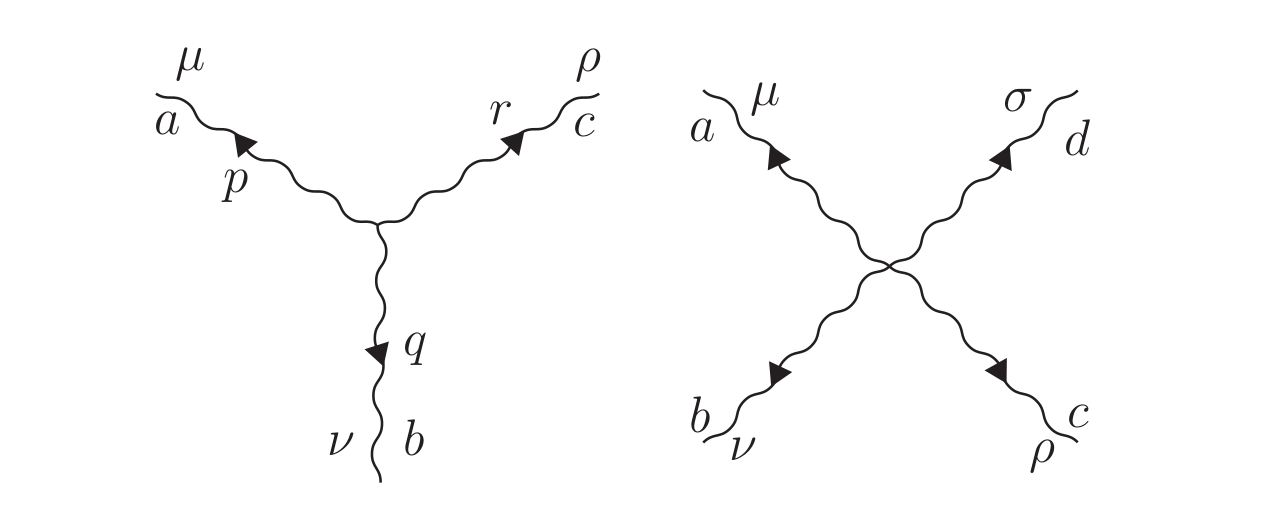
\includegraphics[scale=0.2]{QFT4/gluon_vertices.png}
	\caption{The three-gluon and four-gluon vertices in nonabelian gauge theory}
\end{figure}

\noindent
For loop calculations, we need to include the ghosts. The ghost Lagrangian is
\[\mathcal{L}_{\rm gh} = -\partial^{\mu}\overline{c}^c \partial_{\mu}c^c + gf^{abc}A^a_{\mu}\partial^{\mu}\overline{c}^b c^c\]
The ghost propagator is
\[D_{\rm F}(k) = \frac{-i\delta^{ab}}{k^2-i\epsilon}\]
Because the ghosts are complex scalars, their propagators carry a charge arrow. 

\begin{figure}[!h]
	\centering
	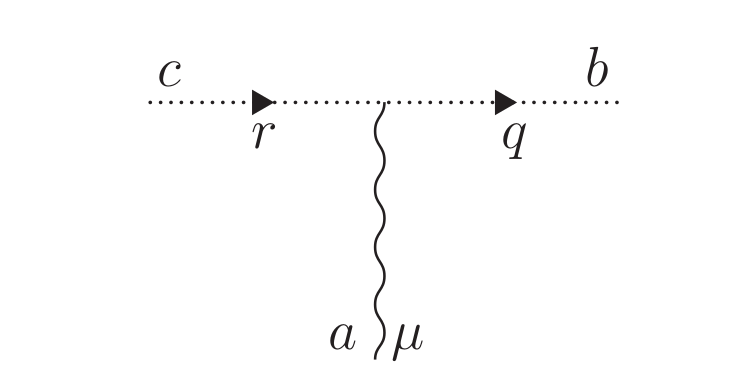
\includegraphics[scale=0.2]{QFT4/ggg_vertex.png}
	\caption{The ghost-ghost-gluon vertex in nonabelian gauge theory}
\end{figure}

\noindent
The ghost–ghost–gluon vertex factor is
\[iV^{abc}_{\mu}(q,r) = igf^{abc}(-iq_{\mu}) = gf^{abc}q_{\mu}\]
If we include a quark coupled to the gluons, we have the quark Lagrangian
\[\mathcal{L}_{q} = i\overline{\Psi}_{i}\slashed{D}_{ij}\Psi_{j} - m\overline{\Psi}_{i}\Psi_{i} = i\overline{\Psi}_{i}\slashed{\partial}\Psi_{i} - m\overline{\Psi}_{i}\Psi_{i} + gA^a_{\mu}\overline{\Psi}_{i} \gamma^{\mu} T^a_{ij} \Psi_j \]

\begin{figure}[!h]
	\centering
	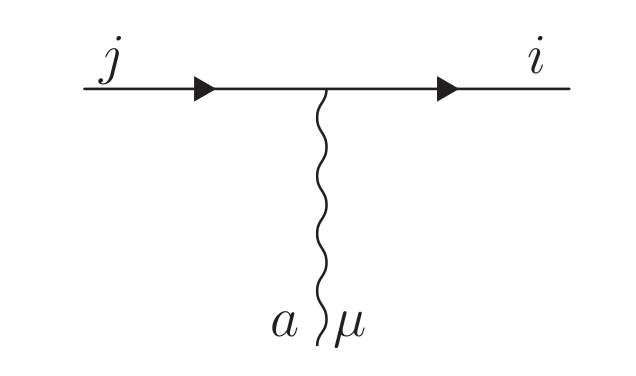
\includegraphics[scale=0.2]{QFT4/ffg_vertex.png}
	\caption{The quark-quark-gluon vertex in nonabelian gauge theory}
\end{figure}

\noindent
The quark propagator is
\[S_F(p)_{ij} = \frac{i(\slashed{p}-m)\delta_{ij}}{p^2+m^2 - i\epsilon}\]
The quark–quark–gluon vertex factor is
\[iV^{\mu a}_{ij} =  ig\gamma^{\mu}T^a_{ij}\]

\section{Renormalization of nonabelian gauge theory}
We now rescale the fields to the renormalized field strengths by extracting the factors $Z_2$, $Z_3$ and $Z_2^c$ for the fermions, gauge bosons, and ghosts, and shift the coupling to the renormalized coupling $g$. The counterterm Lagrangian then takes the form
\begin{eqnarray}
\mathcal{L}_{ct} &=& -\frac{1}{4}\delta_3 F^{a\mu\nu}F^a_{\mu\nu} + \overline{\Psi}(i\delta_2\slashed{\partial}-\delta_m)\Psi + \delta_2^c \overline{c}^a \partial^2 c^a \nonumber \\
&+& g\delta_1 A^a_{\mu}\overline{\Psi}\gamma^{\mu}T^a\Psi -g\delta_{1}^{3g} f^{abe}A^{a\mu}A^{b\nu}\partial_{\mu}A^e_{\nu} - \frac{1}{4}g^2\delta_1^{4g} f^{abe}f^{cde}A^{a\mu}A^{b\nu}A^c_{\mu}A^d_{\nu} \nonumber \\
&+& g\delta_1^c f^{abc}A^a_{\mu}\partial^{\mu}\overline{c}^b c^c \nonumber
\end{eqnarray}
with the counterterms de ned by
\[\delta_2 = Z_2 - 1 \quad \delta_3 = Z_3 - 1 \quad \delta_2^c = Z_2^c - 1 \quad \delta_m = Z_2m_0-m\]
\[\delta_1 = \frac{g_0}{g}Z_2(Z_3)^{1/2} - 1 \quad \delta_1^{3g} = \frac{g_0}{g}(Z_3)^{3/2} - 1 \quad \delta_1^{4g} = \frac{g_0^2}{g^2}(Z_3)^2 - 1 \quad \delta_1^c = \frac{g_0}{g}Z_2^c(Z_3)^{1/2} - 1\]
Notice that these eight counterterms depend on five underlying parameters; thus, there are three relations among them. The situation is very similar to that for the scalar theories with spontaneously broken symmetry that we studied before. 
The underlying symmetry of the theory - local gauge invariance - implies relations among the divergent amplitudes of the theory and among the counterterms required to cancel them. 
In the present case, a set of five renormalization conditions uniquely specifies all of the counterterms in a way that removes all divergences from the theory.
The rigorous proof will be omitted here.

\subsubsection{Quark propagator}
\begin{figure}[!h]
	\centering
	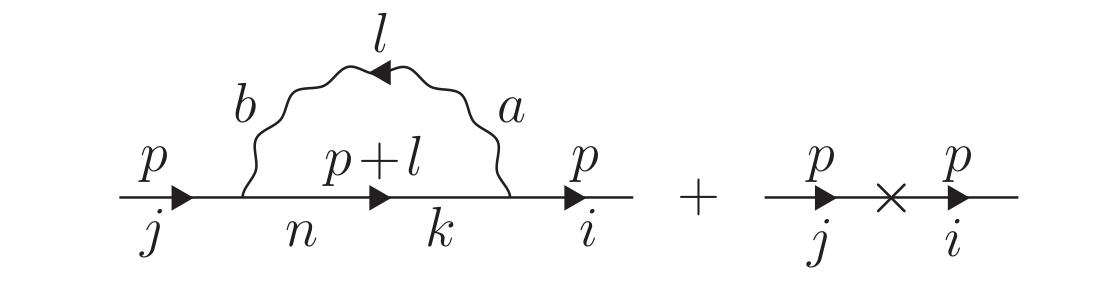
\includegraphics[height=2.96cm ,width=11cm]{QFT4/loop1.png}
	\caption{The one-loop and counterterm corrections to the quark propagator in quantum chromodynamics}
\end{figure}

\noindent
In $\overline{MS}$ renormalization scheme and Feynman gauge, we have
\[Z_2 = 1 - C(R)\frac{g^2}{8\pi^2}\frac{1}{\epsilon} + O(g^4)\]
\[Z_m = 1 - C(R)\frac{g^2}{2\pi^2}\frac{1}{\epsilon} + O(g^4)\]

\subsubsection{Quark-quark-gluon vertex}
\begin{figure}[!h]
	\centering
	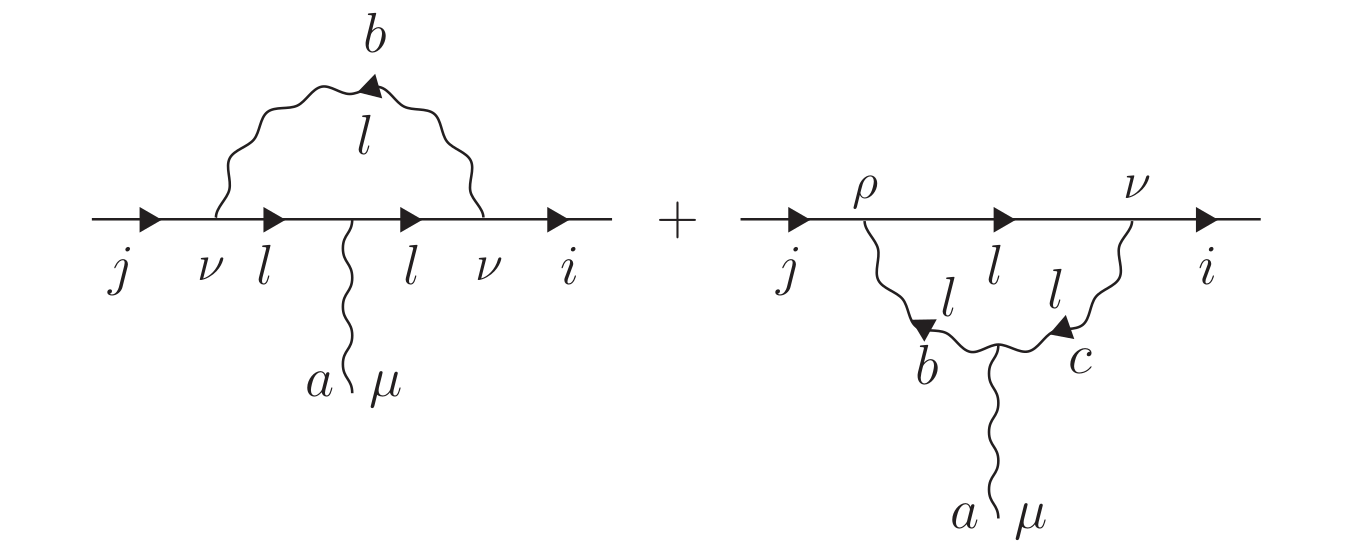
\includegraphics[height=4cm ,width=9.78cm]{QFT4/loop2.png}
	\caption{The one-loop corrections to the quark–quark–gluon vertex in quantum chromodynamics.}
\end{figure}
\[Z_1 = 1 - [C(R) + T(A)]\frac{g^2}{8\pi^2}\frac{1}{\epsilon} + O(g^4)\]

\subsubsection{Gluon propagator}
\begin{figure}[!h]
	\centering
	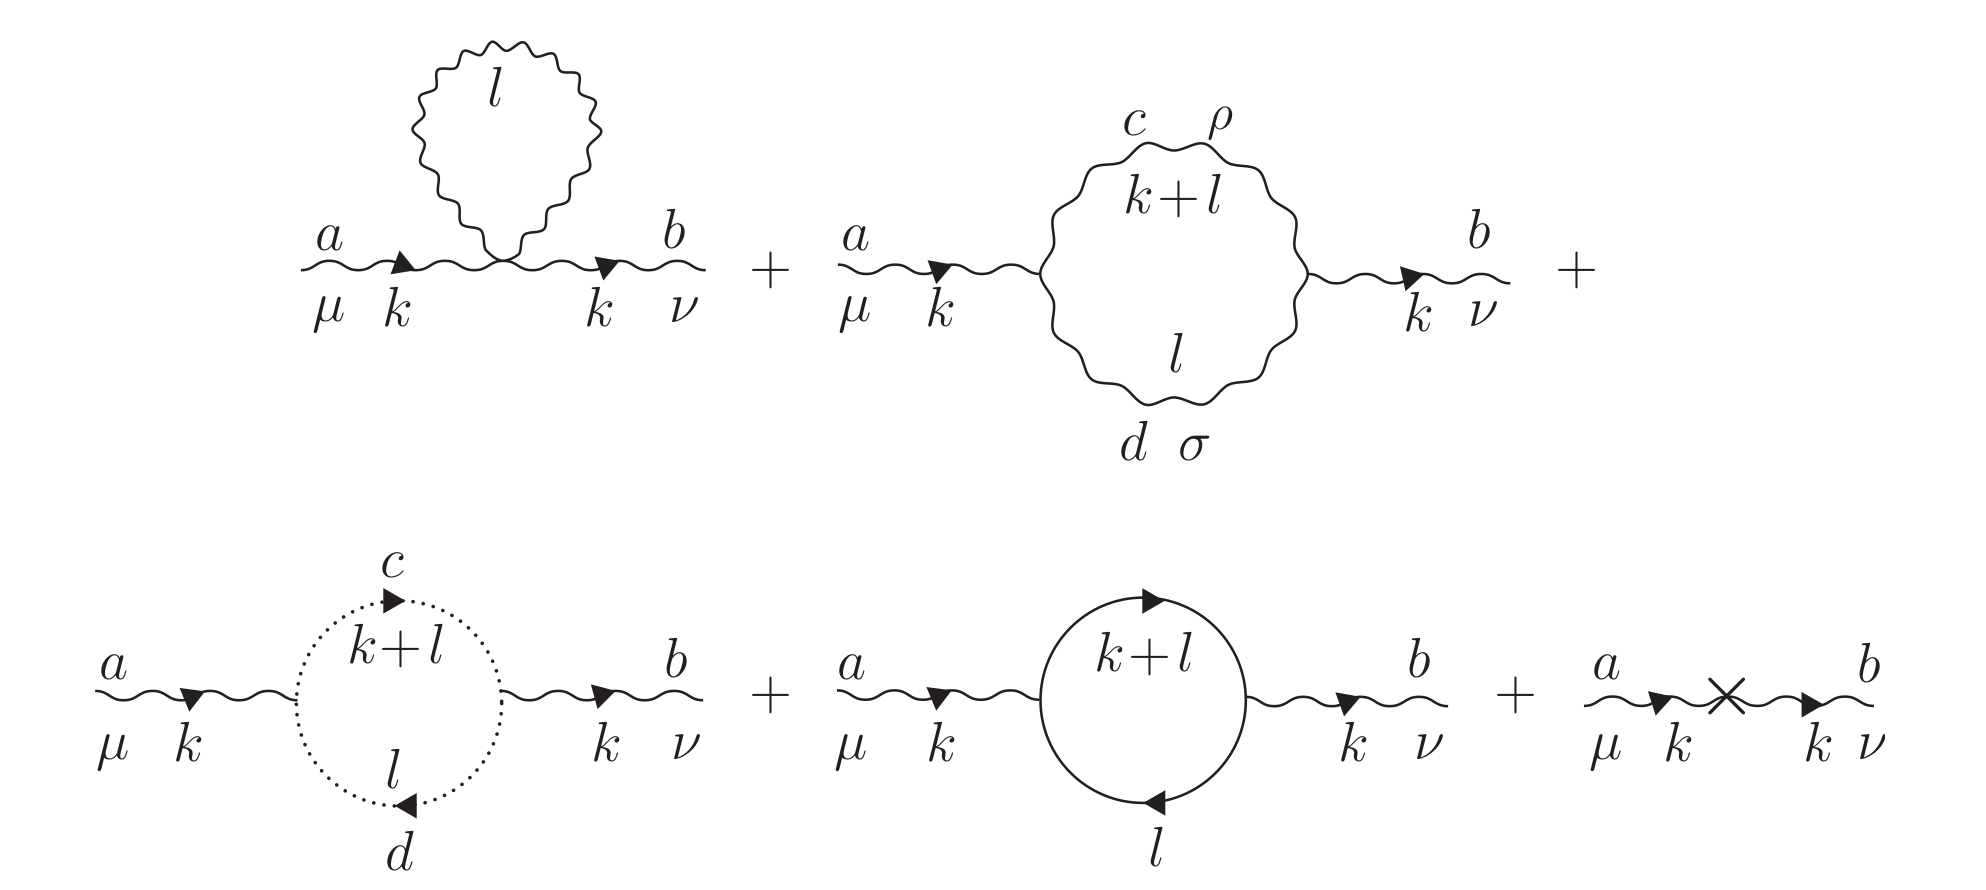
\includegraphics[height=6cm ,width=13.4cm]{QFT4/loop3.png}
	\caption{The one-loop and counterterm corrections to the gluon propagator in quantum chromodynamics.}
\end{figure}
\[Z_3 = 1 + \left[\frac{5}{3}T(A) - \frac{4}{3}n_F T(R)\right]\frac{g^2}{8\pi^2}\frac{1}{\epsilon} + O(g^4)\]

\subsubsection{Beta function}
We define
\[\alpha \equiv \frac{g^2}{4\pi}\]
Then we have
\[\alpha_0 = \frac{Z_1^2}{Z_2^2 Z_3} \alpha \tilde{\mu}^{\epsilon}\]
Let us write
\[\ln \left( Z_3^{-1}Z_2^{-2}Z_1^2 \right) = \sum_{n=1}^{\infty} \frac{G_n(\alpha)}{\epsilon^n}\]
Then we have
\[\ln \alpha_0 = \sum_{n=1}^{\infty} \frac{G_n(\alpha)}{\epsilon^n} + \ln \alpha + \epsilon \ln \tilde{\mu}\]
And we can get
\[G_1(\alpha) = - \left[ \frac{11}{3}T(A) - \frac{4}{3} n_F T(R) \right] \frac{\alpha}{2\pi} + O(\alpha^2)\]
Since the bare coefficients is independent of $\mu$, we then can get
\[\beta(\alpha) = \alpha^2 G_1(\alpha) = - \left[ \frac{11}{3}T(A) - \frac{4}{3} n_F T(R) \right] \frac{\alpha^2}{2\pi} + O(\alpha^3)\]
In quantum chromodynamics, the gauge group is $\mathrm{SU}(3)$, and the quarks are in the fundamental representation. Thus $T(A) = 3$ and $T(R) = \frac{1}{2}$, and the factor in square brackets is $11 - \frac{2}{3} n_F$. So for $n_F \leq 16$, the beta function is negative: the gauge coupling in quantum chromodynamics gets weaker at high energies, and stronger at low energies.\\
This has dramatic physical consequences. Perturbation theory cannot serve as a reliable guide to the low-energy physics. And indeed, in nature we do not see isolated quarks or gluons. (Quarks, in particular, have fractional electric charges and would be easy to discover.) The appropriate conclusion is that color is confined : all finite-energy states are invariant under a global $\mathrm{SU}(3)$ transformation. This has not yet been rigorously proven, but it is the
only hypothesis that is consistent with all of the available theoretical and experimental information.

\section{Chiral gauge theories and anomalies}
\subsection{Chiral gauge theories}
Recall that a Dirac field $\Psi$ can be written in terms of two left-handed Weyl ields $\chi$ and $\xi$ as
\[\Psi = \begin{pmatrix}\chi\\ \xi^{\dagger} \end{pmatrix}\] If $\Psi$ is in a representation $R$ of the gauge group, then $\chi$ and $\xi^{\dagger}$ must be as well. Equivalently, $\chi$ must be in the representation $R$, and $\xi$ must be in the complex conjugate representation $\overline{R}$.
\\
Now suppose that we have a single left-handed Weyl field $\psi$ in a complex representation $R$. Such a gauge theory is automatically parity violating (because the right-handed hermitian conjugate of the left-handed Weyl field is in an inequivalent representation of the gauge group), and is said to be chiral.
The Lagrangian is
\[\mathcal{L} = i\psi^{\dagger} \overline{\sigma}^{\mu} D_{\mu} \psi - \frac{1}{4}F^{a\mu\nu}F^a_{\mu\nu}\]
where $D_{\mu} = \partial_{\mu} - igA^{a}_{\mu} T^a_{\rm R}$.
\\
Since $T^a_{\rm R}$ is a hermitian matrix, $i\psi^{\dagger} \overline{\sigma}^{\mu} D_{\mu} \psi$ is hermitian (up to a total divergence). We cannot include a mass term for $\psi$, though, because $\psi\psi$ transforms as $R \otimes R$, and $R \otimes R$ does not contain a singlet if $R$ is complex. Thus, $\psi\psi$ is not gauge invariant. 
\\ \\
Now we focus on the simplest possible example: a $U(1)$ theory with a single Weyl field $\psi$ with charge $+1$. The Lagrangian is
\[\mathcal{L} = i\psi^{\dagger} \overline{\sigma}^{\mu} (\partial_{\mu} - igA_{\mu}) \psi - \frac{1}{4}F^{\mu\nu}F_{\mu\nu}\]
We note that
\[P_{\mathrm{L}} \Psi = \begin{pmatrix}
\psi \\ 0
\end{pmatrix}\]
Then we can write
\[\mathcal{L} = i\overline{\Psi} \gamma^{\mu} (\partial_{\mu} - igA_{\mu}) P_{\mathrm{L}}\Psi - \frac{1}{4}F^{\mu\nu}F_{\mu\nu}\]
To better understand the physical consequences of the projection operator, consider the case of a free field. The mode expansion is
\[P_{\mathrm{L}}\Psi(x) = \sum_{s = \pm} \int \tilde{dp} [b_s(\bm{p})P_{\mathrm{L}}u_s(\bm{p})e^{ipx} + d_s^{\dagger}(\bm{p})P_{\mathrm{L}} v_s(\bm{p}) e^{-ipx}]\]
For a massless field, we have $P_{\mathrm{L}} u_{+}(\bm{p}) = 0$ and $P_{\mathrm{L}} v_-(\bm{p}) = 0$. Thus we can write as
\[P_{\mathrm{L}}\Psi(x) =  \int \tilde{dp} [b_-(\bm{p})u_-(\bm{p})e^{ipx} + d_+^{\dagger}(\bm{p}) v_+(\bm{p}) e^{-ipx}]\]
We can easily read the Feynman rules from the Lagrangian. In particular, the fermion propagator in momentum space is
\[\frac{iP_{\mathrm{L}}\slashed{p}}{p^2-i\epsilon}\]
and the fermion-fermion-photon vertex is
\[ig\gamma^{\mu} P_{\mathrm{L}}\]
\\
Now consider the correction to the photon propagator. Calculation shows that at the one-loop level, the contribution to $\Pi^{\mu\nu}(k)$ of a single charged Weyl field is half that of a Dirac field. This is physically reasonable, since a Dirac field is equivalent to two charged Weyl fields.
\\
Nothing interesting happens in the one-loop corrections to the fermion propagator, or the fermion-fermion-photon vertex. There is simply an extra factor of $P_{\mathrm{L}}$ along the fermion line, which can be moved to the far right. Except for this factor, the results exactly duplicate those of spinor electrodynamics.
\\
All of this implies that a single Weyl field makes half the contribution of a Dirac field to the leading term in the beta function for the gauge coupling.
\\ \\
Next we turn to diagrams with three external photons, and no external fermions. In spinor electrodynamics, the fact that the vector potential is odd under charge conjugation implies that the sum of these diagrams must vanish. For the present case of a single Weyl field, there is no charge-conjugation symmetry, and so we must evaluate these diagrams.
\begin{figure}[!h]
	\centering
	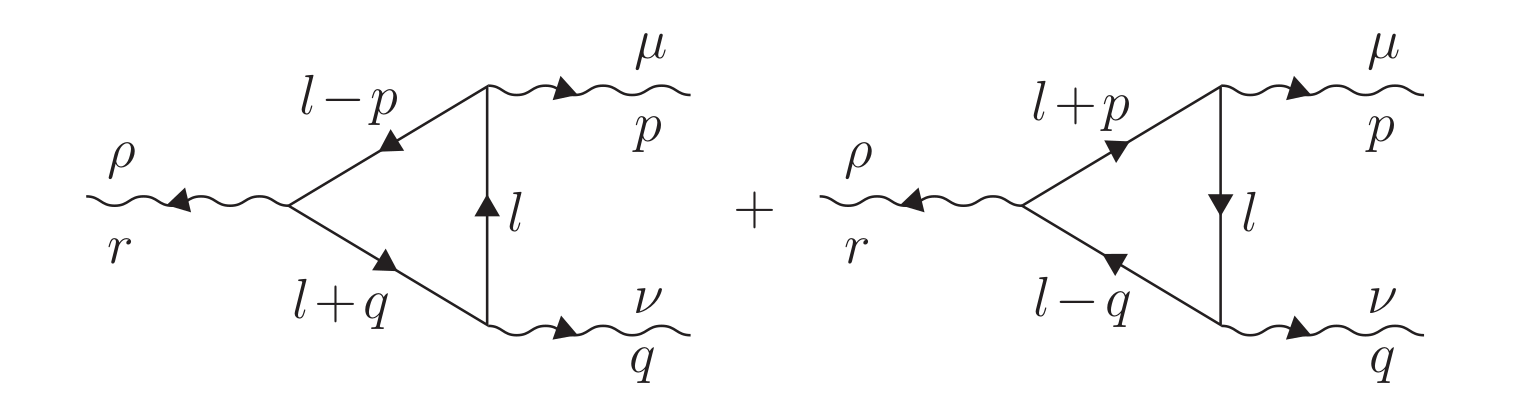
\includegraphics[scale=0.2]{QFT4/chiral1.png}
	\caption{One-loop contributions to the three-photon vertex}
\end{figure}

\noindent
Detailed calculation shows that
\[r_{\rho}V^{\mu\nu\rho}(p,q,r) = 0\]
However,
\[p_{\mu}V^{\mu\nu\rho}(p,q,r) = \frac{ig^3}{8\pi^2}\epsilon^{\alpha\nu\beta\rho}p_{\alpha}q_{\beta}\]
\[q_{\nu}V^{\mu\nu\rho}(p,q,r) = \frac{ig^3}{8\pi^2}\epsilon^{\alpha\rho\beta\mu}q_{\alpha}p_{\beta}\]
We have therefore failed to construct a gauge-invariant $U(1)$ theory with a single charged Weyl field.
\\ \\
Consider now a $U(1)$ gauge theory with several left-handed Weyl fields $\psi_i$, with charges $Q_i$, so that the covariant derivative of $\psi_i$ is $\partial_{\mu} - igQ_iA_{\mu}$. Then each of these fields circulates in the loop in figure above, and each vertex has an extra factor of $Q_i$. The right-hand sides of equation above are now multiplied by $\sum_i Q_i^3$. And if $\sum_i Q_i^3$ happens to be zero, then gauge invariance is restored. 
\\
The simplest possibility is to have the $\psi$s come in
pairs with equal and opposite charges. But there are other possibilities as well: for example, one field with charge $+2$ and eight with charge $-1$. Such a gauge theory is still chiral, but it is anomaly free.
\\ \\
All of this has a straightforward generalization to nonabelian gauge theories. 
Suppose we have a single Weyl field in a (possibly reducible) representation $R$ of the gauge group. Then we must attach an extra factor of $\mathrm{Tr}(T^a_{\rm R} T^b_{\rm R} T^c_{\rm R})$ to the first diagram, and a factor of $\mathrm{Tr}(T^a_{\rm R} T^c_{\rm R} T^b_{\rm R})$ to the second; here the group indices $a,b,c$ go along with the momenta $p,q,r$, respectively.
Repeating our analysis shows that the diagrams with $P_{\mathrm{L}} \to \frac{1}{2}$ come with an extra factor of $\frac{1}{2}\mathrm{Tr}([T^a_{\rm R}, T^b_{\rm R}] T^c_{\rm R})$; these contribute to the renormalization of the tree-level three-gluon vertex. Diagrams with $P_{\mathrm{L}} \to - \frac{1}{2}\gamma_5$ come with an extra factor of
\[\frac{1}{2}\mathrm{Tr}(\{T^a_{\rm R}, T^b_{\rm R}\} T^c_{\rm R}) = A(R)d^{abc}\]
Here $d^{abc}$ is a completely symmetric tensor that is independent of the representation, and $A(R)$ is the anomaly coefficient of $R$. In order for this theory to exist, we must have $A(R) = 0$. 
Since $A(R) + A(\overline{R}) = 0$; thus a theory whose left-handed Weyl fields come in $R \oplus \overline{R}$ pairs is automatically anomaly free (as is one whose Weyl fields are all in real representations). Otherwise, we must arrange the cancellation by hand. 
\\
For $\mathrm{SU}(2)$ and $\mathrm{SO}(N)$, $N \neq 2,6$ all representations have $A(R) = 0$. For $\mathrm{SU}(N)$ with $N \geq 3$, the fundamental representation has $A(N) = 1$, and most complex $\mathrm{SU}(N)$ representations $R$ have $A(R) \neq 0$. So the cancellation is nontrivial.

\subsection{Anomalies in global symmetries}
Let us consider electrodynamics with a massless Dirac field. The Lagrangian is
\[\mathcal{L} = i\overline{\Psi}\slashed{D}\Psi - \frac{1}{4}F^{\mu\nu}F_{\mu\nu}\]
We can write $\Psi$ in terms of two left-handed Weyl fields $\chi$ and $\xi$ via
\[\Psi = \begin{pmatrix}
\chi \\ \xi^{\dagger}
\end{pmatrix}\]
In terms of $\chi$ and $\xi$, the Lagrangian is
\[\mathcal{L} = i\chi^{\dagger}\overline{\sigma}^{\mu} (\partial_{\mu} - igA_{\mu})\chi + i\xi^{\dagger}\overline{\sigma}^{\mu} (\partial_{\mu} + igA_{\mu})\xi\]
Because the fermion field is massless, the Lagrangian is  invariant under a global symmetry in which $\chi$ and $\xi$ transform with the same phase
\[\chi(x) \to e^{i\alpha}\chi(x) \quad \xi(x) \to e^{i\alpha}\xi(x)\]
In terms of $\Psi$, this is
\[\Psi(x) \to e^{-i\alpha\gamma_5}\Psi(x) \quad \overline{\Psi}(x) \to \overline{\Psi} e^{-i\alpha\gamma_5}\]
This is called axial $U(1)$ symmetry, because the associated Noether current
\[j^{\mu}_A = \overline{\Psi}(x) \gamma^{\mu} \gamma_5 \Psi(x)\]
is an axial vector. Noether’s theorem leads us to expect that this current is conserved. However, we will show that the axial current actually has an anomalous divergence.
\\ \\
Consider the matrix element $\langle p,q | j^{\rho}_A(z) |  0 \rangle$, where $\langle p,q |$ is a state of two outgoing photons with four-momenta $p$ and $q$, and polarization vectors $\epsilon_{\mu}$ and $\epsilon'_{\nu}$, respectively. Using the LSZ formula for photons, we have
\[\langle p,q | j^{\rho}_A(z) |  0 \rangle = (ig)^2 \epsilon_{\mu} \epsilon'_{\nu} \int d^4x d^4y e^{-i(px+qy)} \langle 0 | T j^{\mu}(x) j^{\nu}(y) j^{\rho}_A(z) | 0 \rangle \]
where
\[j^{\mu} = \overline{\Psi}\gamma^{\mu}\Psi\]
Let us define $C^{\mu\nu\rho}(p,q,r)$ via
\[(2\pi)^4 \delta(p+q+r)C^{\mu\nu\rho}(p,q,r) \equiv  \int d^4x d^4y d^4z e^{-i(px+qy+rz)} \langle 0 | T j^{\mu}(x) j^{\nu}(y) j^{\rho}_A(z) | 0 \rangle\]
Then we have
\[\langle p,q | j^{\rho}_A(z) |  0 \rangle = -g^2 \epsilon_{\mu} \epsilon'_{\nu} \left. C^{\mu\nu\rho}(p,q,r) e^{irz} \right|_{r=-q-p}\]
Taking the divergence of the current yields
\[\langle p,q | \partial_{\rho} j^{\rho}_A(z) |  0 \rangle = -ig^2 \epsilon_{\mu} \epsilon'_{\nu} r_{\rho} \left. C^{\mu\nu\rho}(p,q,r) e^{irz} \right|_{r=-q-p}\]
We compute $C^{\mu\nu\rho}(p,q,r)$ with Feynman diagrams. At the one-loop level, the contributing diagrams are exactly those we computed in previous subsection, except that the three vertex factors are now $\gamma^{\mu}$, $\gamma^{\nu}$ and $\gamma^{\rho}\gamma_5$ instead of $ig\gamma^{\mu}P_{\mathrm{L}}$, $ig\gamma^{\nu}P_{\mathrm{L}}$ and $ig\gamma^{\rho}P_{\mathrm{L}}$. But, as we saw, the three $P_{\mathrm{L}}$s can be combined into just one at the last vertex, and then this one can be replaced by $-\frac{1}{2}\gamma_5$ . Thus, the vertex function $iV^{\mu\nu\rho}(p,q,r)$ is related to $C^{\mu\nu\rho}(p,q,r)$ by
\[iV^{\mu\nu\rho}(p,q,r) = -\frac{1}{2}(ig)^3 C^{\mu\nu\rho}(p,q,r) + O(g^5)\]
We could choose a regularization scheme that
preserved $p_{\mu}C^{\mu\nu\rho}(p,q,r) = 0$ and $q_{\nu}C^{\mu\nu\rho}(p,q,r) = 0$ but not also $r_{\rho}C^{\mu\nu\rho}(p,q,r) = 0$. This results in
\[r_{\rho}C^{\mu\nu\rho}(p,q,r) = -\frac{i}{2\pi^2} \epsilon^{\mu\nu\alpha\beta} p_{\alpha} q_{\beta} + O(g^2)\]
So, we have
\[\langle p,q | j^{\rho}_A(z) |  0 \rangle  = - \frac{g^2}{2\pi^2} \epsilon^{\mu\nu\alpha\beta} p_{\alpha} q_{\beta} \epsilon_{\mu} \epsilon'_{\nu} e^{-i(p+q)z} + O(g^4) \]
The right-hand side of the equation is exactly what we get in free-field theory for the matrix element of
\[- \frac{g^2}{16\pi^2} \epsilon^{\mu\nu\rho\sigma}F_{\mu\nu}F_{\rho\sigma} + O(g^4) \]
In the next section, we will see the relation is exact.

\subsection{Anomalies and the path integral for fermions}
We begin with the path integral over the Dirac field, with the gauge field treated as a fixed background, to be integrated later. We have
\[Z(A) \equiv \int \mathcal{D}\Psi \mathcal{D}\overline{\Psi} e^{iS(A)}\]
where
\[S(A) \equiv \int d^4x \overline{\Psi}i\slashed{D}\Psi \]
is the Dirac action, $i\slashed{D} = i\gamma^{\mu} D_{\mu}$
is the Dirac operator, and
\[D_{\mu} = \partial_{\mu} - igA_{\mu}\]
is the covariant derivative. Here $A_{\mu}$ is either the $U(1)$ gauge field, or the matrix-valued nonabelian gauge field, depending on the theory under consideration.
\\
Now consider an axial $U(1)$ transformation of the Dirac field, but with a space-time dependent parameter $\alpha(x)$
\[\Psi(x) \to e^{-i\alpha(x)\gamma_5}\Psi(x) \quad \overline{\Psi}(x) \to \overline{\Psi} e^{-i\alpha(x)\gamma_5}\]
The corresponding change in the action is
\[S(A) \to S(A) + \int d^4x j^{\mu}_A(x) \partial_{\mu}\alpha(x) = S(A) - \int d^4x \alpha(x) \partial_{\mu}j^{\mu}_A(x) \]
If we assume that the measure $\mathcal{D}\Psi \mathcal{D}\overline{\Psi}$ is invariant under the axial $U(1)$ transformation, then we have
\[Z(A) = \int \mathcal{D}\Psi \mathcal{D}\overline{\Psi} e^{iS(A)} e^{-i \int d^4x \alpha(x)\partial_{\mu}j^{\mu}_A(x) }\]
This implies that $\partial_{\mu}j^{\mu}_A(x) = 0$ holds inside quantum correlation functions, up to contact terms.
\\ \\
However, the assumption that the measure $\mathcal{D}\Psi \mathcal{D}\overline{\Psi}$ is invariant under the axial $U(1)$ transformation must be examined more closely. The change of variable is implemented by the functional matrix
\[J(x,y) = \delta(x-y)e^{-i\alpha(x)\gamma_5} \]
Because the path integral is over fermionic variables (rather than bosonic), we get a jacobian factor of $(\det J)^{-1}$ (rather than $\det J$) for each of the transformations, so that we have
\[\mathcal{D}\Psi \mathcal{D}\overline{\Psi} \to (\det J)^{-2}\mathcal{D}\Psi \mathcal{D}\overline{\Psi}\]
Using $\log \det J = \mathrm{Tr} \log J$, we can write
\[(\det J)^{-2} = \exp \left[2i \int d^4x \alpha(x) \mathrm{Tr}\delta(x-x)\gamma_5 \right]\]
where the explicit trace is over spin and group indices. We regularize the delta function by
\[\delta(x-y) \to e^{(i\slashed{D}_x)^2/M^2} \delta(x-y)\]
The following calculation can be found in section 77 of \emph{Quantum Field Theory (Mark Srednichi)}. Here, we list the final result
\[\mathrm{Tr} \delta(x-y)\gamma_5 \to - \frac{g^2}{32\pi^2} \epsilon^{\mu\nu\rho\sigma} \mathrm{Tr} F_{\mu\nu}F_{\rho\sigma}\]
We then have
\[Z(A) = \int \mathcal{D}\Psi \mathcal{D}\overline{\Psi} e^{iS(A)} e^{-i \int d^4x \alpha(x)[ \frac{g^2}{16\pi^2} \epsilon^{\mu\nu\rho\sigma} \mathrm{Tr} F_{\mu\nu}F_{\rho\sigma} \partial_{\mu}j^{\mu}_A(x)] }\]
So
\[\partial_{\mu} j^{\mu}_A = -\frac{g^2}{16\pi^2} \epsilon^{\mu\nu\rho\sigma} \mathrm{Tr} F_{\mu\nu}F_{\rho\sigma}\]
is exact. This result is known as the Adler–Bardeen theorem.

\section{Spontaneous breaking of gauge symmetries}
Consider scalar electrodynamics, specified by the Lagrangian
\[\mathcal{L} = -(D_{\mu}\phi)^{\dagger}D_{\mu}\phi - V(\phi) - \frac{1}{4}F^{\mu\nu}F_{\mu\nu}\]
where $\phi$ is a complex scalar field, $D_{\mu} = \partial_{\mu} - ieA_{\mu}$ , and
\[V(\phi) = m^2\phi^{\dagger}\phi + \frac{1}{4}\lambda (\phi^{\dagger}\phi)^2\]
Let us consider $m^2 < 0$. Classically, the field has a nonzero vacuum expectation value (VEV for short), given by
\[\langle 0 | \phi(x) | 0 \rangle = \frac{1}{\sqrt{2}}v\]
where we have made a global $U(1)$ transformation to set the phase of the VEV to zero, and
\[v = \sqrt{\frac{4|m|^2}{\lambda}}\]
We therefore write
\[\phi(x) = \frac{1}{\sqrt{2}} (v + \rho(x)) e^{-i\chi(x)/v}\]
where $\rho(x)$ and $\chi(x)$ are real scalar fields. The scalar potential depends only on $\rho$, and is given by
\[V = \frac{1}{4}\lambda v^2\rho^2 + \frac{1}{4}\lambda v \rho^3 + \frac{1}{16}\lambda \rho^4\]
Since $\chi$ does not appear in the potential, it is massless; it is the Goldstone boson for the spontaneously broken $U(1)$ symmetry.
We can make a gauge transformation that shifts the phase of $\phi(x)$ by an arbitrary space-time function.
We can use this gauge freedom to set $\chi(x) = 0$; this choice is called unitary gauge.
We have
\[-(D_{\mu}\phi)^{\dagger}D_{\mu}\phi = -\frac{1}{2}\partial^{\mu}\rho \partial_{\mu}\rho - \frac{1}{2}g^2(v+\rho)^2 A^{\mu}A_{\mu}\]
We see that the gauge field now has a mass
\[M = gv\]
This is the Higgs mechanism: the Goldstone boson disappears, and the gauge field acquires a mass. Note that this leaves the counting of particle spin states unchanged: a massless spin-one particle has two spin states, but a massive
one has three. The Goldstone boson has become the third or longitudinal state of the now-massive gauge field. A scalar field whose VEV breaks a gauge symmetry is generically called a Higgs field.
\\ \\
This generalizes in a straightforward way to a nonabelian gauge theory. Consider a complex scalar field $\phi$ in a representation $R$ of the gauge group.
The kinetic term for φ is $-(D_{\mu}\phi)^{\dagger}D_{\mu}\phi$, where the covariant derivative is $D_{\mu}\phi_i = \partial_{\mu}\phi_i - igA^a_{\mu}(T^a_{\rm R})_{i}^{\phantom{i}j} \phi_j$ , and the indices $i$ and $j$ run from $1$ to $d(R)$.
We assume that $\phi$ acquires a VEV
\[\langle 0 | \phi_i(x) | 0 \rangle = \frac{1}{\sqrt{2}}v_i\]
If we replace $\phi$ by its VEV in $-(D_{\mu}\phi)^{\dagger}D_{\mu}\phi$, we find a mass term for the gauge fields
\[\mathcal{L}_{mass} = - \frac{1}{2}(M^2)^{ab}A^{a\mu}A^b_{\mu}\]
where the mass-squared matrix is
\[(M^2)^{ab} = g^2 v_i^* (T^a_{\rm R} T^b_{\rm R})_{ij}v_j \]
If the field $\phi$ is real rather than complex (which is possible only if $R$ is a real representation), then we remove the factor of root-two from the right-hand side of vacuum expectation value of $\phi$, but this is compensated by an extra factor of one-half from the kinetic term for a real scalar field; thus the form of mass-squared matrix remains invariant.
\\
We say a generator $T^a$ is spontaneously broken if $(T^a_{\rm R})_{ij}v_j \neq 0$. We see that gauge fields corresponding to broken generators get a mass, while those corresponding to unbroken generators do not. The unbroken generators (if any) form a gauge group with massless gauge fields. The massive gauge fields (and all other fields) form
representations of this unbroken group.
\\ \\
Consider the gauge group $\mathrm{SU}(N)$, with a complex scalar field $\phi$ in the fundamental representation. We can make a global $\mathrm{SU}(N)$ transformation to bring the VEV entirely into the last component, and furthermore make it real. 
Any generator $(T^a)_{i}^{\phantom{j}}$ that does not have a nonzero entry in the last column will remain unbroken. These generators form an unbroken $\mathrm{SU}(N-1)$ gauge group. There are three classes of broken generators: those with $(T^a)_{i}^{\phantom{N}} = \frac{1}{2}$  for $i \neq N$ (there are $N-1$ of these); those with
$(T^a)_{i}^{\phantom{N}} = -\frac{i}{2}$  for $i \neq N$ (there are also $N - 1$ of these), and finally the single
generator $T^{N^2 - 1} = [2N(N-1)]^{-1/2} \mathrm{diag}(1,1,\cdots,-N-1)$. 
\\
The gauge fields corresponding to the generators in the first two classes get a mass $M = \frac{1}{2}gv$.
we can group them into a complex vector field that transforms in the fundamental representation of the unbroken $\mathrm{SU}(N-1)$ subgroup. The gauge field corresponding to $T^{N^2-1}$ gets a mass $M = [2N(N-1)]^{1/2}gv$; it is a singlet of $\mathrm{SU}(N-1)$.
\\ \\
Consider the gauge group $\mathrm{SO}(N)$, with a real scalar field in the fundamental representation. We can make a global $\mathrm{SO}(N)$ transformation to bring the VEV entirely into the last component. Any generator $(T^a)_{i}^{\phantom{j}}$ that does not have a nonzero entry in the last column will remain unbroken. These generators form an unbroken $\mathrm{SO}(N-1)$ subgroup. There are $N - 1$ broken generators, those with $(T^a)_{i}^{\phantom{N}} = -i$  for $i \neq N$. 
The corresponding gauge fields get a mass $M = gv$; they form a fundamental representation of the unbroken $\mathrm{SO}(N-1)$ subgroup.
\\ \\
Consider the gauge group $\mathrm{SU}(N)$, with a real scalar field $\Phi$ a in the adjoint representation. It will prove more convenient to work with the $N \times N$ matrix-valued field $\Phi = \phi^a T^a$; the covariant derivative of $\Phi$ is $D_{\mu}\Phi = \partial_{\mu}\Phi - igA^a_{\mu}[T^a,\Phi]$,
and the VEV of $\phi$ is a traceless hermitian $N \times N$ matrix $V$. Thus the mass squared matrix for the gauge fields is
\[-2g^2 \mathrm{Tr}\left([T^a,V][T^b,V]\right)\]
We can make a global $\mathrm{SU}(N)$ transformation to bring $V$ into diagonal form. Suppose the diagonal entries consist of $N_1$ $v_1$s, followed by $N_2$ $v_2$s, etc.,
where $v_1 < v_2 < \cdots$ and $\sum_i N_i v_i = 0$. 
Then all generators whose nonzero entries lie entirely within the $i$th block commute with $V$, and hence form an
unbroken $\mathrm{SU}(N_i)$ subgroup. Furthermore, generators that is proportional to $V$ also commutes with $V$, and forms a
$U(1)$ subgroup. Thus the unbroken gauge group is $\mathrm{SU}(N_1)\times \mathrm{SU}(N_2) \times \cdots \times U(1)$. The gauge coupling constants for the different groups are all the same, and equal to the original $\mathrm{SU}(N)$ gauge coupling constant.
\\ \\
\begin{example}
Consider the case of $\mathrm{SU}(5)$, which has $24$ generators. Let the diagonal entries of $V$ be given by $(-\frac{1}{3},-\frac{1}{3},-\frac{1}{3}, \frac{1}{2}, \frac{1}{2})$. The unbroken subgroup is then $\mathrm{SU}(3) \times \mathrm{SU}(2) \times U(1)$. The number of broken generators is $24 - 8 - 3 - 1 = 12$.
\end{example}

\section{Quantization of spontaneously broken gauge theory}
\subsection{Spontaneously broken abelian gauge theory}
Consider scalar electrodynamics, specified by the Lagrangian
\[\mathcal{L} = -(D_{\mu}\phi)^{\dagger}D_{\mu}\phi - V(\phi) - \frac{1}{4}F^{\mu\nu}F_{\mu\nu}\]
where $\phi$ is a complex scalar field, $D_{\mu} = \partial_{\mu} - ieA_{\mu}$. We choose
\[V(\phi) = \frac{1}{4}\lambda (\phi^{\dagger}\phi - \frac{1}{2}v^2)^2\]
which yields a nonzero VEV for $\phi$. We therefore write
\[\phi = \frac{1}{\sqrt{2}}(v + h + ib)\]
where $h$ and $b$ are real scalar fields. In terms of $h$ and $b$, the potential is
\[V = \frac{1}{4}\lambda v^2 h^2 + \frac{1}{4}\lambda vh(h^2+b^2) + \frac{1}{16}\lambda (h^2+b^2)^2\]
The covariant derivative term can be expanded as
\begin{eqnarray}
-(D_{\mu}\phi)^{\dagger}D_{\mu} = &-& \frac{1}{2}\partial_{\mu}h \partial^{\mu}h -  \frac{1}{2}\partial_{\mu}b \partial^{\mu}b - \frac{1}{2} g^2v^2A^{\mu}A_{\mu} + gv A^{\mu}\partial_{\mu}b \nonumber \\
&+& gA^{\mu} (h\partial_{\mu}b - b\partial_{\mu}h) - gvhA^{\mu}A_{\mu} - \frac{1}{2}g^2(h^2+b^2)A^{\mu}A_{\mu} \nonumber
\end{eqnarray}
The first line contains all the terms that are quadratic in the fields. The first two are the kinetic terms for the $h$ and $b$ fields. The third is the mass term for the vector field. The fourth is an annoying cross term between the vector field and the derivative of $b$.
\\ \\
In abelian gauge theory, in the absence of spontaneous symmetry breaking, we fix gauge by adding to $\mathcal{L}$ the gauge-fixing and ghost terms
\[\mathcal{L}_{gf} + \mathcal{L}_{gh} = - \frac{G^2}{2\xi} - \overline{c}\frac{\delta G}{\delta \theta} c \]
where $G = \partial^{\mu}A_{\mu}$, and $\theta(x)$ parameterizes an infinitesimal gauge transformation
\[A_{\mu} \to A_{\mu} - \partial_{\mu}\theta \quad \phi \to ig\theta\phi\]
Since $\delta G / \delta \theta = - \partial^2$, the ghost fields have no interactions, and can be ignored.
\\ \\
In the presence of spontaneous symmetry breaking, we choose instead
\[G = \partial^{\mu}A_{\mu} - \xi g\nu b\]
which reduces to $\partial^{\mu}A_{\mu}$ when $v = 0$. Multiplying out $G^2$ , we have
\[\mathcal{L}_{gf} = -\frac{1}{2\xi} \partial^{\mu}A_{\mu} \partial^{\nu}A_{\nu} - gvA_{\mu}\partial^{\mu}b - \frac{1}{2}\xi g^2v^2b^2\]
Note that the second term cancels the annoying cross term between the vector field and the derivative of $b$. Also, the last term on the gives a mass $\sqrt{\xi}M$ to the $b$ field ( $M = gv$).
\\ \\
We must still evaluate $\mathcal{L}_{gh}$. To do so, we note under gauge transformation,
\[h \to h + g\theta b \quad b \to b - g\theta(v+h)\]
Then we have
\[\frac{\delta G}{\delta \theta} = -\partial^2 + \xi g^2 v(v+h)\]
The ghost Lagrangian is
\[\mathcal{L}_{gh} = -\partial^{\mu}\overline{c}\partial_{\mu}c - \xi g^2v^2\overline{c}c - \xi g^2 vh\overline{c}c\]
We see from the second term that the ghost has acquired the same mass as the $b$ field.
\\ \\
Now let us examine the vector field. Including $\mathcal{L}_{gh}$, the terms that are quadratic in the vector field can be written as
\[\mathcal{L}_0 = - \frac{1}{2}A_{\mu} \left[ \eta^{\mu\nu}(-\partial^2 + M^2) + (1 - \xi)\partial^{\mu}\partial^{\nu} \right] A_{\nu}\]
The propagator for vector field is
\[S_F(k) = \frac{-iP^{\mu\nu}}{k^2+M^2-i\epsilon} + \frac{\xi k^{\mu}k^{\nu}/k^2}{k^2+ \xi M^2-i\epsilon}\]
where $P^{\mu\nu} = g^{\mu\nu} - k^{\mu}k^{\nu}/k^2$ projects onto the transverse subspace. We see that the transverse components of the vector field propagate with mass $M$, while the longitudinal component propagates with the same mass as the $b$ and ghost fields, $\sqrt{\xi}M$.
\\ \\
Since their masses depend on $\xi$, the ghosts, the $b$ field, and the longitudinal component of the vector field must all represent unphysical particles that do not appear in incoming or outgoing states. When $\xi \to \infty$, we can recover the unitary gauge. The details can be found in section 76 of \emph{Quantum Field Theory (Mark Srednichi)}.

\subsection{Spontaneously broken nonabelian gauge theory}
It will be convenient to work with real scalar fields. We
therefore decompose any complex scalar fields into pairs of real ones, and organize all the real scalar fields into a big list $\phi_i$, $i = 1,\cdots,N$. 
These real scalar fields form a (possibly reducible) representation $R$ of the gauge group. Let $T^a$ be the gauge-group generator matrices; they are linear combinations of the generators of the $\mathrm{SO}(N)$ group that rotates all components of $\phi_i$ into each other. Because these generators are hermitian and antisymmetric, so are the  $T^A$s. The Lagrangian for our theory can now be written as
\[\mathcal{L} = -\frac{1}{2}D^{\mu}\phi D_{\mu}\phi - V(\phi) - \frac{1}{4}F^{a\mu\nu}F^a_{\mu\nu}\]
where
\[(D_{\mu}\phi)_i = \partial_{\mu}\phi_i - ig_aA^a_{\mu}T^a_{ij}\phi_j\]
is the covariant derivative.
\\
Now we suppose that the potential is minimized when $\phi$ has a VEV
\[\langle 0 | \phi_i | 0 \rangle = v_i\]
A generator $T^a$ is unbroken if $T^a_{ij}v_j = 0$, and broken if $T^a_{ij}v_j \neq 0$.
\\ \\
Each broken generator results in a massless Goldstone boson. We note that the potential must be invariant under a global gauge transformation, so
\[\frac{\partial V}{\partial \phi_j} T^a_{jk}\phi_k = 0\]
We differentiate it with respect to $\phi_i$ to get
\[\frac{\partial^2 V}{\partial \phi_i \partial \phi_j} T^a_{jk}\phi_k + \frac{\partial V}{\partial \phi_j} T^a_{ji} = 0 \]
Now set $\phi_i = v_i$; then $\frac{\partial V}{\partial \phi_i}$ vanishes. Also, we can identify
\[(m^2)_{ij} = \left. \frac{\partial^2 V}{\partial \phi_i \partial \phi_j} \right|_{\phi_i = v_i}\]
as the mass-squared matrix for the scalars (after spontaneous symmetry breaking). Thus we have
\[(m^2)_{ij} (T^av)_j = 0\]
We see that if $T^av \neq 0$, then $T^av$ is an eigenvector of the mass-squared matrix with eigenvalue zero. So there is a zero eigenvalue for every linearly independent broken generator.
\\ \\
Let us write
\[\phi_i(x) = v_i + \chi_i(x)\]
The covariant derivative of becomes
\[(D_{\mu}\phi)_i = \partial_{\mu}\chi_i - ig_aA^a_{\mu}T^a_{ij}(v+\chi)_j\]
It is now convenient to define a set of real antisymmetric matrices
\[\tau^a_{ij} \equiv ig_aT^a_{ij}\]
and the real rectangular matrix
\[F^a_{\phantom{i}i} \equiv \tau^a_{ij}v_j\]
We can now write
\[(D_{\mu}\phi)_i = \partial_{\mu}\chi_i - A^a_{\mu}(F^a+\tau^a\chi)_i\]
The kinetic term for $\phi$ becomes
\begin{eqnarray}
-\frac{1}{2}D^{\mu}\phi D_{\mu}\phi = &-& \frac{1}{2}\partial_{\mu}\chi_i \partial^{\mu}\chi_i - \frac{1}{2}(F^a_{\phantom{i}i} F^b_{\phantom{i}i})A^{a\mu}A^b_{\mu} + F^a_{\phantom{i}i} A^a_{\mu}\partial^{\mu}\chi_i \nonumber \\
&+& A^a_{\mu}\chi_i \tau^a_{ij}\partial^{\mu}\chi_j - A^{a\mu}A^b_{\mu} F^a_{\phantom{i}i} \tau^b_{ij} \chi_j - \frac{1}{2}A^{a\mu}A^b_{\mu}\chi_i (\tau^a \tau^b)_{ij}\chi_j \nonumber
\end{eqnarray}
We see that the mass-squared matrix for the vector fields is
\[(M^2)^{ab} = F^a_{\phantom{i}i} F^b_{\phantom{i}i} = (FF^T)^{ab}\]
A theorem of linear algebra states that every real rectangular matrix can be written as
\[F^a_{\phantom{i}i} = S^{ac}(M^c\delta^c_{\phantom{i}j})R_{ji}\]
where $S$ and $R$ are orthogonal matrices, and the diagonal entries $M^c$ are real and nonnegative. We see that these diagonal entries are the masses of the vector fields. The vector fields of definite mass are then given by $\widetilde{A}^{a}_{\mu} = S^{ba}A^b_{\mu}$.
\\ \\
Now we are ready to fix $R_{\xi}$ gauge. To do so, we add to $\mathcal{L}$ the gauge-fixing and ghost terms
\[\mathcal{L}_{gf} + \mathcal{L}_{gh} = - \frac{G^aG^a}{2\xi} - \overline{c}^a\frac{\delta G^a}{\delta \theta^b} c^b \]
where we choose
\[G^a = \partial^{\mu}A^a_{\mu} - \xi F^a_{\phantom{i}i} 
\chi_i\]
Then we have
\[\mathcal{L}_{gf} = -\frac{1}{2\xi} \partial^{\mu}A^a_{\mu} \partial^{\nu}A^a_{\nu} - F^a_{\phantom{i}i} A^a_{\mu}\partial^{\mu}\chi_i - \frac{1}{2}\xi (F^a_{\phantom{i}i} F^a_{\phantom{i}j})\chi_i\chi_j\]
The last term makes a contribution to the mass-squared matrix for the $\chi$ fields,
\[\xi(M^2)_{ij} = \xi F^a_{\phantom{i}i} F^a_{\phantom{i}j} = \xi(F^TF)_{ij}\]
The eigenvalues of this matrix are $\sqrt{\xi}M^a$ , where
$M^a$ are the vector-boson masses. The mass-squared matrix $\xi M^2$ should be added to the mass-squared matrix $m^2$ that we get from the potential. We can verify that
\[(m^2)_{ij}(\xi M^2)_{jk} = 0\]
Thus these two contributions to the mass-squared matrix of the scalar fields live in orthogonal subspaces. The $m^2$ subspace consists of the physical, massive scalars, and the $\xi M^2$ subspace consists of the unphysical Goldstone bosons; these are the fields that would be set to zero in unitary gauge.
\\ \\
Finally, we must evaluate $\mathcal{L}_{gh}$. Under an infinitesimal gauge transformation, we have
\[ A^a_{\mu} \to A^a_{\mu} - D^{\mu}_{ab}\theta^b \quad \chi_i \to \chi_i - \theta^a \tau^a_{ij}(v+\chi)_j \]
Thus we have
\[\frac{\delta G^a}{\delta \theta^b} = - D^{\mu}_{ab} + \xi(M^2)^{ab} + \xi F^a_{\phantom{i}j} \tau^b_{jk}\chi_k \]
and so the ghost lagrangian is
\[\mathcal{L}_{gh} = -\partial^{\mu} \overline{c}^a D_{\mu}^{ab} c^b - \xi (M^2)^{ab}\overline{c}^a c^b - \xi F^a_{\phantom{i}j} \tau^b_{jk}\chi_k \overline{c}^a c^b\]
The ghost fields of definite mass are $\widetilde{c}^a = S^{ba}c^b$ and  $\widetilde{\overline{c}}^a = S^{ba}\overline{c}^b$.

\section{The Standard Model}
\subsection{Gauge and Higgs sector}
We begin with the electroweak part of the gauge group, $\mathrm{SU}(2)\times U(1)$, and the complex scalar field $\phi$, known as the Higgs field, in the representation $(2,-\frac{1}{2})$. The Higgs field acquires a non-zero VEV that spontaneously breaks $\mathrm{SU}(2)\times U(1)$ to $U(1)$; the unbroken $U(1)$ is identified as electromagnetism.
We begin with the covariant derivative of the Higgs field $\phi$,
\[(D_{\mu}\phi)_i = \partial_{\mu}\phi_i - i[g_2 A^a_{\mu}T^a + g_1B_{\mu}Y]_{i}^{\phantom{i}j} \phi_j\] where $T^a = \frac{1}{2}\sigma^a$ and $Y = -\frac{1}{2}I$; $Y$ is the hypercharge generator. It will prove
useful to write out $g_2 A^a_{\mu}T^a + g_1B_{\mu}Y$ in matrix form,
\[ \frac{1}{2} \begin{pmatrix}
g_2A^3_{\mu}-g_1B_{\mu} & g_2(A^1_{\mu} - iA^2_{\mu}) \\
g_2(A^1_{\mu} + iA^2_{\mu}) & -g_2A^3_{\mu}-g_1B_{\mu}
\end{pmatrix}\]
Now suppose that $\phi$ has a potential
\[V(\phi) = \frac{1}{4}\lambda (\phi^{\dagger}\phi - \frac{1}{2}v^2)^2\]
This potential gives $\phi$ a non-zero VEV. We can make a global gauge transformation to bring this VEV entirely into the first component, and furthermore make it real, so that
\[\langle 0 | \phi | 0 \rangle =  \frac{1}{\sqrt{2}}\begin{pmatrix}
v \\ 0
\end{pmatrix} \]
The kinetic term for $\phi$ is $-(D_{\mu}\phi)^{\dagger}D_{\mu}\phi$. After replacing $\phi$ by its VEV, we find a mass term for the gauge fields,
\[\mathcal{L}_{\mathrm{mass}}  = - \frac{1}{8}v^2 \begin{pmatrix}
1 & 0 \end{pmatrix} \begin{pmatrix}
g_2A^3_{\mu}-g_1B_{\mu} & g_2(A^1_{\mu} - iA^2_{\mu}) \\
g_2(A^1_{\mu} + iA^2_{\mu}) & -g_2A^3_{\mu}-g_1B_{\mu}
\end{pmatrix}^2 \begin{pmatrix} 1 \\ 0 \end{pmatrix} \]
Define the weak mixing angle
\[\theta_{\mathrm{W}} \equiv \tan^{-1}(g_1/g_2)\]
and the fields
\begin{eqnarray}
W^{\pm}_{\mu} &\equiv & \frac{1}{\sqrt{2}} (A^1_{\mu} \mp iA^2_{\mu}) \nonumber \\
Z_{\mu}  &\equiv & c_{\mathrm{W}} A^3_{\mu} - s_{\mathrm{W}} B_{\mu} \nonumber \\
A_{\mu}  &\equiv & s_{\mathrm{W}} A^3_{\mu} + c_{\mathrm{W}} B_{\mu} \nonumber
\end{eqnarray}
where $c_{\mathrm{W}} \equiv \cos \theta_{\mathrm{W}}$ and $s_{\mathrm{W}} \equiv \sin \theta_{\mathrm{W}}$. 
In terms of these fields, we have
\[\mathcal{L}_{\mathrm{mass}} = -M_{\mathrm{W}}^2 W^{+\mu} W^{-}_{\mu} - \frac{1}{2}M_{\mathrm{Z}}^2 Z^{\mu}Z_{\mu}\]
where we have identified
\[M_{\mathrm{W}} \equiv \frac{g_2v}{2} \quad M_{\mathrm{Z}} \equiv \frac{M_{\mathrm{W}}}{\cos\theta_{\mathrm{W}}}\]
Note that the $A_{\mu}$ field remains massless; this signifies that there is an unbroken $U(1)$ subgroup. We will identify this unbroken $U(1)$ with the gauge
group of electromagnetism.
\\ \\
The two complex components of the $\phi$ field yield four real scalar fields; three of these become the longitudinal components of the $W^{\pm}$ and $Z^0$. The remaining scalar field must be able to account for shifts in the overall scale of $\phi$. Thus we can write, in unitary gauge,
\[\phi(x) = \frac{1}{\sqrt{2}} \begin{pmatrix}
v + H(x) \\ 0
\end{pmatrix}\]
where $H$ is a real scalar field; the corresponding particle is the Higgs boson. The potential now reads
\[V = \frac{1}{4}\lambda v^2H^2 + \frac{1}{4}\lambda v H^3 + \frac{1}{16}\lambda H^4\]
We see that the mass of the Higgs boson is given by $m_{\mathrm{H}}^2 = \frac{1}{2}\lambda v^2$. The kinetic term for $H$ comes from the kinetic term for $\phi$, and is the usual one for a real scalar field, $-\frac{1}{2}\partial_{\mu}H \partial^{\mu}H$. Finally, recall that the mass term for the gauge fields is proportional to $v^2$. Hence it should be multiplied by a factor of $(1 + \frac{H}{v})^2$.
\\ \\
Now we have to work out the kinetic terms for the gauge fields. We have
\[\mathcal{L} = -\frac{1}{4}F^{a\mu\nu}F^a_{\mu\nu} - \frac{1}{4}B^{\mu\nu}B_{\mu\nu}\]
We find
\[\frac{1}{\sqrt{2}} (F^1_{\mu\nu} - iF^2_{\mu\nu}) = D_{\mu} W^+_{\nu} - D_{\nu}W^+_{\mu}\]
\[\frac{1}{\sqrt{2}} (F^1_{\mu\nu} + iF^2_{\mu\nu}) = D_{\mu} W^-_{\nu} - D_{\nu}W^-_{\mu}\]
where we have defined a covariant derivative that acts on
$W^+$,
\[D_{\mu} \equiv \partial_{\mu} - ig_2A^3_{\mu} = \partial_{\mu} - ig_2(s_{\mathrm{W}}A_{\mu} + c_{\mathrm{W}} Z_{\mu})\]
If we identify $A_{\mu}$ as the electromagnetic vector potential, and assign electric charge $Q = +1$ (in units of the proton charge) to the $W^+$, then we must identify the electromagnetic coupling constant $e$ as
\[e \equiv g_2 s_{\mathrm{W}}\]
Here we are adopting the convention that $e$ is positive. (In our treatment of quantum electrodynamics, we used the convention that $e$ is negative, but that is less convenient in the present context.)
We also have
\[F^3_{\mu\nu} = s_{\mathrm{W}}F_{\mu\nu} + c_{\mathrm{W}} Z_{\mu\nu} -ig_2(W_{\mu}^+ W_{\nu}^- - W_{\nu}^+ W_{\mu}^-)\]
\[B_{\mu\nu} = c_{\mathrm{W}}F_{\mu\nu} - s_{\mathrm{W}} Z_{\mu\nu}\]
where $F_{\mu\nu} = \partial_{\mu}A_{\nu} - \partial_{\nu}A_{\mu}$ is the usual electromagnetic field strength, and
\[Z_{\mu\nu} \equiv \partial_{\mu}Z_{\nu} - \partial_{\nu}Z_{\mu}\]
is the abelian field strength associated with the $Z_{\mu}$ field.
\\ \\
Now we can assemble all of this into the complete Lagrangian for the electroweak gauge fields and the Higgs boson in unitary gauge. We will express $g_2$ in terms of $e$ and $\theta_{\mathrm{W}}$, and $\lambda$ in terms of $m_{\mathrm{H}}$ and
$v$. We ultimately get
\begin{eqnarray}
\mathcal{L} = &-& \frac{1}{4} F_{\mu\nu}F^{\mu\nu} - \frac{1}{4} Z_{\mu\nu}Z^{\mu\nu} - D^{\dagger\mu}W^{-\nu}D_{\mu}W^{+}_{\nu} + D^{\dagger\mu}W^{-\nu}D_{\nu}W^{+}_{\mu} \nonumber \\
&+& ie(F^{\mu\nu} + \cot\theta_{\mathrm{W}} Z^{\mu\nu})W_{\mu}^+ W_{\nu}^- \nonumber \\
&-& \frac{1}{2} \frac{e^2}{\sin^2\theta_{\mathrm{W}}} (W^{+\mu}W_{\mu}^{-}W^{+\nu}W_{\nu}^{-} -W^{+\mu}W_{\mu}^{+}W^{-\nu}W_{\nu}^{-} ) \nonumber \\
&-& (M_{\mathrm{W}}^2 W^{+\mu} W^{-}_{\mu} + \frac{1}{2}M_{\mathrm{Z}}^2 Z^{\mu}Z_{\mu})(1 + \frac{H}{v})^2 \nonumber \\
&-& \frac{1}{2}\partial_{\mu}H \partial^{\mu}H  - \frac{1}{2}m_{\mathrm{H}}^2 H^2  - \frac{1}{2}m_{\mathrm{H}}^2 v^{-1} H^3 -  \frac{1}{8}m_{\mathrm{H}}^2 v^{-2}H^4 \nonumber
\end{eqnarray}
where
\[D_{\mu} = \partial_{\mu} -ie(A_{\mu} + \cot\theta_{\mathrm{W}}Z_{\mu})\]

\subsection{Lepton sector}
Leptons are spin-one-half particles that are singlets of the color group. There are six different flavours of lepton. The six flavours are naturally grouped into three families or generations: $e$ and $\nu_e$, $\mu$ and $\nu_{\mu}$, $\tau$ and $\nu_{\tau}$.
\\ \\
Let us begin by describing a single lepton family, the electron and its neutrino. We introduce left-handed Weyl fields $l$ and $\bar{e}$ in the representations $(2,-\frac{1}{2})$ and $(1,+1)$ of $\mathrm{SU}(2)\times U(1)$. 
Here the bar over the $e$ in the field $\bar{e}$ is part of the name of the field, and does not denote any sort of conjugation. The covariant derivatives of these fields are
\[(D_{\mu}l)_i = \partial_{\mu}l_i - ig_2A^a_{\mu}(T^a)_{i}^{\phantom{j}j}l_j - ig_1(-\frac{1}{2})B_{\mu}l_i\]
\[D_{\mu}\bar{e} = \partial_{\mu}\bar{e} - ig_1(+1)B_{\mu}\bar{e}\]
and their kinetic terms are
\[\mathcal{L}_{\mathrm{kin}} = il^{\dagger i} \overline{\sigma}^{\mu}(D_{\mu}l)_i + i\bar{e}^{\dagger}\overline{\sigma}^{\mu}D_{\mu}\bar{e}\]
We cannot write down a mass term involving $l$ and(or) $\bar{e}$ because there is no gauge-group singlet contained in any of the products
\[(2,-\frac{1}{2}) \otimes (2,-\frac{1}{2}) \quad (2,-\frac{1}{2}) \otimes (1, +1) \quad (1, +1) \otimes (1, +1)\]
However, we are able to write down a Yukawa coupling of the form
\[\mathcal{L}_{\mathrm{Yuk}} \equiv -y\epsilon^{ij}\phi_i l_j \bar{e} + \mathrm{h.c.}\]
where $\phi$ is the Higgs field in the $(2,-\frac{1}{2})$ representation, and $y$ is the Yukawa coupling constant. A gauge-invariant Yukawa coupling is possible because there is a singlet on the right-hand side of
\[(2,-\frac{1}{2}) \otimes (2,-\frac{1}{2}) \otimes (1,+1) = (1,0) \oplus (3,0)\]
In unitary gauge, we replace $\phi_1$ with $\frac{1}{\sqrt{2}}(v+H)$, where $H$ is the real scalar field representing the physical Higgs boson, and $\phi_2$ with zero. The Yukawa term becomes
\[\mathcal{L}_{\mathrm{Yuk}} = -\frac{1}{\sqrt{2}}y(v+H)(l_2\bar{e} + \mathrm{h.c.})\]
It is now convenient to assign new names to the $\mathrm{SU}(2)$ components of $l$,
\[l = \begin{pmatrix}
\nu \\ e
\end{pmatrix} \]
So, we have
\[\mathcal{L}_{\mathrm{Yuk}} = -\frac{1}{\sqrt{2}}y(v+H)\overline{\mathcal{E}}\mathcal{E}\]
where we have defined a Dirac field for the electron
\[\mathcal{E} \equiv \begin{pmatrix}
e \\ \bar{e}^{\dagger}
\end{pmatrix} \]
We see that the electron has acquired a mass $m_e \equiv \frac{yv}{\sqrt{2}}$, while neutrino has remained massless.
We can describe the neutrino with a Majorana field
\[\mathcal{N} \equiv \begin{pmatrix}
\nu \\ \nu^{\dagger}
\end{pmatrix}\]
However, it is often more convenient to work with
\[\mathcal{N}_{\mathrm{L}} \equiv P_{\mathrm{L}} \mathcal{N} = \begin{pmatrix}
\nu \\ 0
\end{pmatrix}\]
We can think of $\mathcal{N}_{\mathrm{L}}$ as a Dirac field; for example, the neutrino kinetic term can be written as $i\overline{\mathcal{N}_{\mathrm{L}}} \slashed{\partial} \mathcal{N}_{\mathrm{L}}$.
\\ \\
Now we express the covariant derivatives in terms of the $W_{\mu}^{\pm}$ , $Z_{\mu}$ , and $A_{\mu}$ fields. We have
\[g_2 A^1_{\mu}T^1 + g_2 A^2_{\mu}T^2 = \frac{g_2}{\sqrt{2}} \begin{pmatrix}
0 & W_{\mu}^+ \\ W^{-}_{\mu} & 0
\end{pmatrix} \]
and
\[g_2A^3_{\mu}T^3 + g_1 B_{\mu} Y = e(T^3+Y)A_{\mu} + e(\cot\theta_{\mathrm{W}} T^3 - \tan\theta_{\mathrm{W}} Y)Z_{\mu}\]
Since we identify $A_{\mu}$ as the electromagnetic field and $e$ as the electromagnetic coupling constant (with the convention that $e$ is positive), we identify
\[Q = T^3 + Y\]
as the generator of electric charge. Then we have
\[Q\nu = 0 \quad Qe = -e \quad Q\bar{e} = +\bar{e}\]
It is convenient to replace $Y$ with $Q - T^3$. We find
\[g_2A^3_{\mu}T^3 + g_1 B_{\mu} Y = eQA_{\mu} + \frac{e}{s_{\mathrm{W}} c_{\mathrm{W}}}( T^3 -  s_{\mathrm{W}}^2Q)Z_{\mu}\]
In terms of the four-component fields, we have
\[(g_2A^3_{\mu}T^3 + g_1 B_{\mu} Y) \mathcal{E} = \left[-eA_{\mu} + \frac{e}{s_{\mathrm{W}} c_{\mathrm{W}}}( -\frac{1}{2}P_{\mathrm{L}} +  s_{\mathrm{W}}^2)Z_{\mu} \right] \mathcal{E}\]
\[(g_2A^3_{\mu}T^3 + g_1 B_{\mu} Y) \mathcal{N}_{\mathrm{L}} = \frac{e}{s_{\mathrm{W}} c_{\mathrm{W}}} (+\frac{1}{2}) Z_{\mu}\mathcal{N}_{\mathrm{L}} \]
The couplings of the gauge fields to the leptons can be written as
\[\mathcal{L}_{\mathrm{int}} = \frac{1}{\sqrt{2}}g_2W_{\mu}^{+} J^{-\mu} + \frac{1}{\sqrt{2}}g_2W_{\mu}^{-} J^{+\mu} +  \frac{e}{s_{\mathrm{W}} c_{\mathrm{W}}} Z_{\mu}J_{\mathrm{Z}}^{\mu} + eA_{\mu}J^{\mu}_{\mathrm{EM}}\] 
where
\begin{eqnarray}
J^{+\mu} &\equiv & \overline{\mathcal{E}}_{\mathrm{L}} \gamma^{\mu} \mathcal{N}_{\mathrm{L}} \nonumber \\
J^{-\mu} &\equiv & \overline{\mathcal{N}}_{\mathrm{L}} \gamma^{\mu} \mathcal{E}_{\mathrm{L}} \nonumber \\
J_{\mathrm{Z}}^{\mu} &\equiv & J_3^{\mu} - s_{\mathrm{W}}^2 J^{\mu}_{\mathrm{EM}} \nonumber \\
J_3^{\mu} &\equiv & \frac{1}{2}\overline{\mathcal{N}}_{\mathrm{L}} \gamma^{\mu} \mathcal{N}_{\mathrm{L}} - \frac{1}{2}\overline{\mathcal{E}}_{\mathrm{L}} \gamma^{\mu} \mathcal{E}_{\mathrm{L}} \nonumber \\
J^{\mu}_{\mathrm{EM}} &\equiv &  -\overline{\mathcal{E}} \gamma^{\mu} \mathcal{E}_{\mathrm{L}} \nonumber
\end{eqnarray}
\\ \\
Having worked out the interactions of a single lepton generation, we now examine what happens when there is more than one of them. 
Let us consider the fields $l_{iI}$ and $\bar{e}_{I}$, where $I=1,2,3$ is a generation index. The kinetic term for all these fields is
\[\mathcal{L}_{\mathrm{kin}} = il^{\dagger i}_I \overline{\sigma}^{\mu}(D_{\mu})_{i}^{\phantom{i}j} l_{jI} + i\bar{e}_I^{\dagger}\overline{\sigma}^{\mu}D_{\mu}\bar{e}_I\]
where the repeated generation index is summed. The most general Yukawa term we can write down now reads
\[\mathcal{L}_{\mathrm{Yuk}} = -\epsilon^{ij}\phi_i l_{jI}y_{IJ} \bar{e}_{J} + \mathrm{h.c.}\]
where $y_{IJ}$ is a complex $3 \times 3$ matrix, and the generation indices are summed.
We can make unitary transformations in generation space on the fields: $l_I \to L_{IJ} l_J$ and $\bar{e}_I \to \overline{E}_{IJ}\bar{e}_J$ , where $L$ and $\overline{E}$ are independent unitary matrices.
The kinetic terms are unchanged, and the Yukawa matrix $y$ is replaced with $L^T y \overline{E} $. We can choose $L$ and $\overline{E}$ so that $L^T y \overline{E}$ is diagonal with positive real entries $y_I$. The charged leptons then have masses $m_{eI} = \frac{y_Iv}{\sqrt{2}}$, and the neutrinos remain massless. In the currents, we simply add a generation index $I$ to each field, and sum over it.

\subsection{Quark sector}
Quarks are spin-one-half particles that are triplets of the color group. There are six different flavours of quark. The six flavours are naturally grouped into three families or generations: $u$ and $d$, $c$ and $s$, $t$ and $b$.
\\ \\
Let us begin by describing a single quark family, the up and down quarks. We introduce left-handed Weyl fields $q$, $\bar{u}$, and $\bar{d}$ in the representations
$(3,2,+\frac{1}{6})$, $(\bar{3},1,-\frac{2}{3})$, and $(\bar{3},1,+\frac{1}{3})$ of $\mathrm{SU}(3) \times \mathrm{SU}(2) \times U(1)$. 
Here the bar over the letter in the fields is part of the name of the field, and does not denote any sort of conjugation
The covariant derivatives of these fields are
\begin{eqnarray}
(D_{\mu}q)_{\alpha i} &=& \partial_{\mu}q_{\alpha i} - ig_3A^a_{\mu}(T^a_3)_{\alpha}^{\phantom{\alpha}\beta} q_{\beta i} - ig_2A^a_{\mu}(T^a_2)_{i}^{\phantom{j}j} q_{\alpha j} - ig_1(+\frac{1}{6})B_{\mu} q_{\alpha i}
\nonumber \\
(D_{\mu}\bar{u})^{\alpha} &=& \partial_{\mu}\bar{u}^{\alpha} -ig_3A^a_{\mu}(T^a_{\bar{3}})^{\alpha}_{\phantom{\alpha}\beta} \bar{u}^{\beta } - ig_1(-\frac{2}{3})B_{\mu}\bar{u}^{\alpha}
\nonumber \\
(D_{\mu}\bar{d})^{\alpha} &=& \partial_{\mu}\bar{d}^{\alpha} -ig_3A^a_{\mu}(T^a_{\bar{3}})^{\alpha}_{\phantom{\alpha}\beta} \bar{d}^{\beta } - ig_1(+\frac{1}{3})B_{\mu}\bar{d}^{\alpha}
\nonumber
\end{eqnarray}
We rely on context to distinguish the $\mathrm{SU}(3)$ gauge fields from the $\mathrm{SU}(2)$ gauge fields. The kinetic terms for $q$, $\bar{u}$, and $\bar{d}$ are
\[\mathcal{L}_{\mathrm{kin}} = iq^{\dagger \alpha i} \overline{\sigma}^{\mu} (D_{\mu}q)_{\alpha i} + i\bar{u}^{\dagger}_{\alpha}\overline{\sigma}^{\mu}(D_{\mu}\bar{u})^{\alpha} + i\bar{d}^{\dagger}_{\alpha}\overline{\sigma}^{\mu}(D_{\mu}\bar{d})^{\alpha}\]
We cannot write down a mass term involving $q$, $\bar{u}$, and/or $\bar{d}$ because there is no gauge-group singlet contained in any of the products of their representations. But we are able to write down Yukawa couplings of the form
\[\mathcal{L}_{\mathrm{Yuk}} = -y'\epsilon^{ij}\phi_i q_{\alpha j} \bar{d}^{\alpha} - y'' \phi^{\dagger i}q_{\alpha i} \bar{u}^{\alpha} + \mathrm{h.c.}\]
where $\phi$ is the Higgs field in the $(1,2,-\frac{1}{2})$ representation, and $y'$ and $y''$ are the Yukawa coupling constants. These gauge invariant Yukawa couplings are possible because there are singlets on the right-hand sides of
\[(1,2,-\frac{1}{2}) \otimes (3, 2, +\frac{1}{6}) \otimes (\bar{3}, 1, +\frac{1}{3}) = (1,1,0) \oplus\]
\[(1,2, \frac{1}{2}) \otimes (3, 2, +\frac{1}{6}) \otimes (\bar{3}, 1, -\frac{2}{3}) = (1,1,0) \oplus\]
In unitary gauge, we replace $\phi_1$ with $\frac{1}{\sqrt{2}}(v+H)$, where $H$ is the real scalar field representing the physical Higgs boson, and $\phi_2$ with zero. The Yukawa term becomes
\[\mathcal{L}_{\mathrm{Yuk}} = -\frac{1}{\sqrt{2}}y'(v+H)q_{\alpha 2}\bar{d}^{\alpha} - \frac{1}{\sqrt{2}}y''(v+H)q_{\alpha 1}\bar{u}^{\alpha} + \mathrm{h.c.}\]
It is now convenient to assign new names to the $\mathrm{SU}(2)$ components of $q$,
\[q = \begin{pmatrix}
u \\ d
\end{pmatrix} \]
Then we have
\[\mathcal{L}_{\mathrm{Yuk}} = -\frac{1}{\sqrt{2}}y'(v+H) \overline{\mathcal{D}}_{\alpha}\mathcal{D}_{\alpha} -\frac{1}{\sqrt{2}}y''(v+H) \overline{\mathcal{U}}_{\alpha}\mathcal{U}_{\alpha}\]
where we have defined Dirac fields for the down and up quarks
\[\mathcal{D}_{\alpha} \equiv \begin{pmatrix}
d_{\alpha} \\ \bar{d}^{\dagger}_{\alpha}
\end{pmatrix} \quad  \mathcal{U}_{\alpha} \equiv \begin{pmatrix}
u_{\alpha} \\ \bar{u}^{\dagger}_{\alpha}
\end{pmatrix}\]
We see  that the up and down quarks have acquired masses
\[m_d \equiv \frac{y'v}{\sqrt{2}} \quad m_u \equiv \frac{y''v}{\sqrt{2}}\]
Now we express the covariant derivatives in terms of the $W_{\mu}^{\pm}$ , $Z_{\mu}$ , and $A_{\mu}$ fields. We have
\[g_2 A^1_{\mu}T^1 + g_2 A^2_{\mu}T^2 = \frac{g_2}{\sqrt{2}} \begin{pmatrix}
0 & W_{\mu}^+ \\ W^{-}_{\mu} & 0
\end{pmatrix} \]
\[g_2A^3_{\mu}T^3 + g_1 B_{\mu} Y = e(T^3+Y)A_{\mu} + e(\cot\theta_{\mathrm{W}} T^3 - \tan\theta_{\mathrm{W}} Y)Z_{\mu}\]
and
\[Q = T^3 + Y\]
We see that
\[Qu = +\frac{2}{3}u \quad Qd = -\frac{1}{3}d \quad Q\bar{u} = -\frac{2}{3}\bar{u} \quad Q\bar{d} = +\frac{1}{3}\bar{d}\]
This is just the set of electric charge assignments that we expect for the up and down quarks. In terms of the four-component fields, we have
\[(g_2A^3_{\mu}T^3 + g_1 B_{\mu} Y) \mathcal{U} = \left[ + \frac{2}{3}eA_{\mu} + \frac{e}{s_{\mathrm{W}} c_{\mathrm{W}}}( \frac{1}{2}P_{\mathrm{L}} -\frac{2}{3}  s_{\mathrm{W}}^2)Z_{\mu} \right] \mathcal{U}\]
\[(g_2A^3_{\mu}T^3 + g_1 B_{\mu} Y) \mathcal{U} = \left[ - \frac{1}{3}eA_{\mu} + \frac{e}{s_{\mathrm{W}} c_{\mathrm{W}}}( -\frac{1}{2}P_{\mathrm{L}} +\frac{1}{3}  s_{\mathrm{W}}^2)Z_{\mu} \right] \mathcal{U}\]
The couplings of the electroweak gauge fields to the quarks is
\[\mathcal{L}_{\mathrm{int}} = \frac{1}{\sqrt{2}}g_2W_{\mu}^{+} J^{-\mu} + \frac{1}{\sqrt{2}}g_2W_{\mu}^{-} J^{+\mu} +  \frac{e}{s_{\mathrm{W}} c_{\mathrm{W}}} Z_{\mu}J_{\mathrm{Z}}^{\mu} + eA_{\mu}J^{\mu}_{\mathrm{EM}}\] 
where we have defined the currents
\begin{eqnarray}
J^{+\mu} &\equiv & \overline{\mathcal{D}}_{\mathrm{L}} \gamma^{\mu} \mathcal{U}_{\mathrm{L}} \nonumber \\
J^{-\mu} &\equiv & \overline{\mathcal{U}}_{\mathrm{L}} \gamma^{\mu} \mathcal{D}_{\mathrm{L}} \nonumber \\
J_{\mathrm{Z}}^{\mu} &\equiv & J_3^{\mu} - s_{\mathrm{W}}^2 J^{\mu}_{\mathrm{EM}} \nonumber \\
J_3^{\mu} &\equiv & \frac{1}{2}\overline{\mathcal{U}}_{\mathrm{L}} \gamma^{\mu} \mathcal{U}_{\mathrm{L}} - \frac{1}{2}\overline{\mathcal{D}}_{\mathrm{L}} \gamma^{\mu} \mathcal{D}_{\mathrm{L}} \nonumber \\
J^{\mu}_{\mathrm{EM}} &\equiv &  +\frac{2}{3}\overline{\mathcal{U}} \gamma^{\mu} \mathcal{U}_{\mathrm{L}} - \frac{1}{3}\overline{\mathcal{D}} \gamma^{\mu} \mathcal{D}_{\mathrm{L}} \nonumber
\end{eqnarray}
Having worked out the interactions of a single quark generation, we now examine what happens when there is more than one of them.
Let us consider the fields $q_{\alpha iI}$, $\bar{u}_{I}$ and $\bar{d}_{I}$, where $I=1,2,3$ is a generation index. The kinetic term for all these fields is
\[\mathcal{L}_{\mathrm{kin}} = iq^{\dagger\alpha i I} \overline{\sigma}^{\mu}(D_{\mu})_{\alpha i}^{\phantom{\alpha i}\beta j} q_{\beta jI} + i\bar{u}_{\alpha I}^{\dagger}\overline{\sigma}^{\mu} (D_{\mu})^{\alpha}_{\phantom{\alpha}\beta}\bar{u}_I^{\beta} + i\bar{d}_{\alpha I}^{\dagger}\overline{\sigma}^{\mu} (D_{\mu})^{\alpha}_{\phantom{\alpha}\beta}\bar{d}_I^{\beta}\]
where the repeated generation index is summed. The most general Yukawa term we can write down now reads
\[\mathcal{L}_{\mathrm{Yuk}} = -\epsilon^{ij}\phi_i q_{\alpha jI}y'_{IJ} \bar{d}^{\alpha}_{J} -\phi^{\dagger i} q_{\alpha jI}y''_{IJ} \bar{u}^{\alpha}_{J} + \mathrm{h.c.}\]
$y'$ and $y''$ are complex $3 \times 3$ matrices. In unitary gauge, this becomes
\[\mathcal{L}_{\mathrm{Yuk}} = -\frac{1}{\sqrt{2}}(v+H) d_{\alpha I}y'_{IJ} \bar{d}^{\alpha}_{J} -\frac{1}{\sqrt{2}}(v+H) u_{\alpha I}y''_{IJ} \bar{u}^{\alpha}_{J} + \mathrm{h.c.}\]
We can make unitary transformations in generation space on the fields: $d_I \to D_{IJ}d_J $, $\bar{d}_I \to \overline{D}_{IJ}\bar{d}_J$, $u_I \to U_{IJ}u_J $ and $\bar{u}_I \to \overline{U}_{IJ}\bar{u}_J$, where $U$, $\overline{U}$, $D$, $\overline{D}$ are independent unitary matrices. 
The kinetic terms are unchanged (except for the couplings to the $W^{\pm}$, as we will discuss momentarily), and the Yukawa matrices $y'$ and $y''$ are replaced with $D^T y' \overline{D}$  and $U^T y'' \overline{U}$ . We can choose
$U$, $\overline{U}$, $D$, $\overline{D}$ so that $D^T y' \overline{D}$  and $U^T y'' \overline{U}$ are diagonal with positive real entries $y'_I$ and $y''_I$. The down quarks $D_I$ then have masses $m_{dI} = \frac{y'_I v}{\sqrt{2}}$,
and the up quarks $u_I$ have masses $m_{uI} = \frac{y''_I v}{\sqrt{2}}$. In the neutral currents, we simply add a generation index $I$ to each field, and sum over it. 
The charged currents are more complicated, however; they become 
\[J^{+\mu} = \overline{\mathcal{D}}_{\mathrm{L}I} (V^{\dagger})_{IJ} \gamma^{\mu} \mathcal{U}_{\mathrm{L}J}\]
\[J^{-\mu} = \overline{\mathcal{U}}_{\mathrm{L}I} V_{IJ} \gamma^{\mu} \mathcal{D}_{\mathrm{L}J}\]
where $V \equiv U^{\dagger} D$ is the Cabibbo-Kobayasi-Maskawa matrix (or CKM matrix for short).
\\
A $3 \times 3$ unitary matrix has nine real parameters. However, we are still free to make the independent phase rotations $\mathcal{D}_I = e^{i\alpha_I} \mathcal{D}_I$ and $\mathcal{U}_I = e^{i\beta_I} \mathcal{U}_I$ , as
these leave the kinetic and mass terms invariant. These phase changes allow us to make the first row and column of $V_{IJ}$ real, eliminating five of the nine parameters. The remaining four can be chosen as $\theta_1$ (the Cabibbo angle),$\theta_2$ ,$\theta_3$ , and $\delta$, where
\[V = \begin{pmatrix}
c_1 & +s_1c_3 & +s_1s_3 \\
-s_1c_2 & c_1c_2c_3 - s_2s_3e^{i\delta} & c_1c_2s_3 + s_2c_3e^{i\delta} \\
-s_1s_2 & c_1s_2c_3 + c_2s_3e^{i\delta} & c_1s_2s_3- c_2c_3 e^{i\delta}
\end{pmatrix} \]
and $c_i = \cos\theta_i$ and $s_i = \sin\theta_i$. The measured values of these angles are $s_1=0.224$, $s_2 = 0.041$, $s_3 = 0.016$ , and $\delta = 40^{\circ}$. Note that the charged currents now have some terms with a phase factor $e^{i\delta}$, and some without. 
Since the time-reversal operator T is antiunitary, the charged currents do not transform in a simple way under time reversal. This implies that the charged current terms in $\mathcal{L}_{\mathrm{int}}$ are not time-reversal invariant; hence the electroweak interactions violate time-reversal symmetry.
Since $CPT$ is always a good symmetry, time-reversal violation is equivalent to $CP$ violation; $\delta$ is therefore sometimes called the $CP$ violating phase.